\def\SigleNumero{STT-2902}
\def\NomCours{Modélisation statistique}

\newcommand{\affichepoints}{.}     % ← AVEC points
% \renewcommand{\affichepoints}{on} % ← SANS points (non vide)

\documentclass{Evaluation}
\usepackage{multicol,graphicx}
\usepackage{fancyvrb}
\usepackage{comment}
\noprintanswers

% ============================================================
% MÉCANISME D'AFFICHAGE CONDITIONNEL DES TITRES DE MODULES
% ============================================================
\makeatletter
\newcommand{\currentmodulekey}{}
\newcommand{\currentmoduletitle}{}
\newcommand{\currentgroupkey}{}
\newcommand{\currentgrouptitle}{}
\newcommand{\modulegroupheader}[2]{%
  \renewcommand{\currentgroupkey}{#1}%
  \renewcommand{\currentgrouptitle}{#2}%
  \expandafter\global\expandafter\let\csname modulegroup@#1@shown\endcsname\relax
}
\newcommand{\moduleheader}[2]{%
  \renewcommand{\currentmodulekey}{#1}%
  \renewcommand{\currentmoduletitle}{#2}%
  \expandafter\global\expandafter\let\csname module@#1@shown\endcsname\relax
}
\newcommand{\showmoduleifneeded}{%
  \ifx\currentgroupkey\empty\else
    \expandafter\ifx\csname modulegroup@\currentgroupkey @shown\endcsname\relax
      \section*{\currentgrouptitle}%
      \expandafter\gdef\csname modulegroup@\currentgroupkey @shown\endcsname{1}%
    \fi
  \fi
  \expandafter\ifx\csname module@\currentmodulekey @shown\endcsname\relax
    \section*{\currentmoduletitle}%
    \expandafter\gdef\csname module@\currentmodulekey @shown\endcsname{1}%
  \fi
}
\makeatother

% ============================================================
% CONFIGURATION DES SESSIONS À AFFICHER
% ============================================================
\newenvironment{A25}{\showmoduleifneeded}{}

% Décommentez pour cacher une session :
%\excludecomment{A25}

% Supprimer la page couverture et ajuster les marges
\renewcommand{\couverture}{\newgeometry{margin=1.7cm,left=0.7cm,bottom=1.5cm,footskip=0mm}}

\begin{document}

\begin{center}
  {\Large\textbf{\SigleNumero\ -- \NomCours}}\\[0.3cm]
  {\large Recueil d'exercices}
\end{center}
\medskip

\begin{questions}

% ============================================================
%        MODULE 1 — STATISTIQUES DESCRIPTIVES
% ============================================================
\moduleheader{mod1}{Statistiques descriptives et échantillonnage}

\begin{A25}
\question Une municipalité souhaite connaître le temps moyen de déplacement domicile-travail de ses \textbf{30\,000 résidents actifs}. Le bureau du transport vous fournit le tableau suivant:

\begin{table}[h]
    \centering
    \begin{tabular}{|c|c|c|c|c|}
    \hline
        Identifiant & Nom, Prénom & Quartier & Mode de transport & Temps (min) \\
        \hline
        1 & Tremblay, Xavier & Centre-ville & Vélo & 12 \\
        \hline
        2 & Lavoie, Marie & Banlieue Nord & Auto & 35 \\
        \hline
        3 & Gagnon, Pierre & Banlieue Sud & Autobus & 48 \\
        \hline
        ... & ... & ... & ... & ... \\
        \hline
    \end{tabular}
\end{table}

Supposez qu'il y a 6 quartiers, chacun contenant 5\,000 résidents. Chaque quartier a 5 secteurs de 1\,000 résidents. Vous souhaitez interroger \textbf{300 résidents}.

\begin{parts}
    \part[3] Expliquez précisément comment vous procéderiez pour utiliser un échantillonnage par grappes.

    \begin{solution}
        On choisit les grappes comme étant les secteurs (30 secteurs au total). On sélectionne un certain nombre de secteurs au hasard (par exemple 3 secteurs parmi 30, par échantillonnage aléatoire simple) et on interroge tous les résidents de chaque secteur sélectionné. Ici, puisque chaque secteur a 1\,000 résidents, il faudra trouver un nombre de grappes qui donne environ 300 résidents, soit une fraction de grappes.

        Autre possibilité: choisir les quartiers comme grappes (6 quartiers). On en choisit quelques-uns et on interroge les $300/k$ résidents dans chacun des $k$ quartiers sélectionnés. L'important est de préciser ce qu'on utilise comme grappes et comment on les sélectionne.
    \end{solution}

    \part[5] Proposez une stratification et expliquez dans quelle situation elle serait avantageuse.

    \begin{solution}
        On pourrait stratifier par \texttt{Mode de transport} (par ex. Vélo, Auto, Autobus, Métro). Cette stratification serait avantageuse si le temps de déplacement est très différent d'un mode de transport à l'autre (forte variabilité inter-strates), mais assez homogène à l'intérieur de chaque mode (faible variabilité intra-strate). Par exemple, les cyclistes ont probablement des temps courts, tandis que les usagers d'autobus ont des temps plus longs et plus variables.
    \end{solution}

    \part[4] On vous dit que la distribution de la variable \texttt{Temps (min)} est fortement asymétrique à droite. Devrait-on utiliser la médiane plutôt que la moyenne pour résumer cette variable? \textit{\textbf{Expliquez.}}

    \begin{solution}
        Oui, la médiane serait plus appropriée dans ce cas. Lorsque la distribution est fortement asymétrique à droite, quelques individus avec des temps de déplacement très longs tirent la moyenne vers le haut, ce qui la rend peu représentative du temps «typique». La médiane, qui n'est pas sensible aux valeurs extrêmes, donnerait une meilleure idée du temps de déplacement d'un résident typique.
    \end{solution}

    \part[3] De quel type est la variable \texttt{Mode de transport}?

    \begin{solution}
        Il s'agit d'une variable qualitative nominale (les catégories n'ont pas d'ordre naturel).
    \end{solution}

    \part[3] Votre collègue propose de calculer la corrélation entre la variable \texttt{Quartier} et la variable \texttt{Temps (min)}. Qu'en pensez-vous?

    \begin{solution}
        La corrélation (de Pearson ou de Spearman) n'est pas appropriée ici, car \texttt{Quartier} est une variable qualitative nominale. La corrélation mesure l'association linéaire entre deux variables quantitatives. On ne peut pas calculer la corrélation avec une variable qualitative nominale.
    \end{solution}

    \part[2] Est-il pertinent de calculer le coefficient de variation de la variable \texttt{Temps (min)}?

    \begin{solution}
        Oui, car la variable \texttt{Temps (min)} est une variable quantitative de rapport (le zéro est un vrai zéro: un temps de 0 minutes signifie aucun déplacement). Le coefficient de variation est pertinent pour ce type de variable.
    \end{solution}
\end{parts}
\end{A25}

\begin{A25}
\question Soit les 15 valeurs suivantes représentant le nombre d'heures d'étude par semaine d'un groupe d'étudiants:

\begin{center}
\begin{tabular}{c c c c c}
2 & 4 & 5 & 7 & 8 \\
8 & 10 & 10 & 12 & 14 \\
15 & 18 & 22 & 30 & 45 \\
\end{tabular}
\end{center}

\begin{parts}
    \part[3] Calculez les quartiles $Q_1$, $Q_2$ (médiane) et $Q_3$.

    \begin{solution}
        Les 15 données sont déjà triées. $Q_2 = x_{(8)} = 10$ (la 8\textsuperscript{e} valeur). $Q_1$ est la médiane de la moitié inférieure (positions 1 à 7): $Q_1 = x_{(4)} = 7$. $Q_3$ est la médiane de la moitié supérieure (positions 9 à 15): $Q_3 = x_{(12)} = 18$.
    \end{solution}

    \part[3] Y a-t-il des valeurs aberrantes selon la règle de 1,5$\times$EIQ? \textit{\textbf{Justifiez.}}

    \begin{solution}
        $\text{EIQ} = Q_3 - Q_1 = 18 - 7 = 11$. Limites: $Q_1 - 1{,}5 \times \text{EIQ} = 7 - 16{,}5 = -9{,}5$ et $Q_3 + 1{,}5 \times \text{EIQ} = 18 + 16{,}5 = 34{,}5$. La valeur $45 > 34{,}5$ est donc une valeur aberrante. Aucune valeur n'est inférieure à $-9{,}5$.
    \end{solution}

    \part[2] Quelle est la forme de cette distribution?

    \begin{solution}
        La distribution est asymétrique à droite (la queue de droite est plus longue, la moyenne est plus grande que la médiane, et on observe une valeur extrême élevée à 45).
    \end{solution}

    \part[2] Laquelle de la moyenne ou de la médiane sera la plus grande?

    \begin{solution}
        La moyenne sera plus grande que la médiane, car la distribution est asymétrique à droite. Les valeurs extrêmes élevées (comme 45) tirent la moyenne vers le haut.
    \end{solution}
\end{parts}
\end{A25}

\begin{A25}
\question Dites si chacun des énoncés suivants est vrai ou faux. \textit{Justifiez brièvement.}

\begin{parts}
    \part[2] La corrélation de Spearman et la corrélation de Pearson donnent toujours le même résultat.

    \begin{solution}
        Faux. La corrélation de Spearman se calcule sur les rangs des données, tandis que la corrélation de Pearson se calcule sur les valeurs brutes. Elles ne donnent le même résultat que si la relation entre les deux variables est parfaitement linéaire croissante ou décroissante. En général, elles sont différentes.
    \end{solution}

    \part[2] Si $X_1,\ldots,X_n$ sont mesurés en kg, alors la variance est en kg$^2$ et l'écart-type est en kg.

    \begin{solution}
        Vrai. La variance est la moyenne des carrés des écarts, donc ses unités sont le carré des unités de la variable. L'écart-type est la racine carrée de la variance, donc il a les mêmes unités que la variable.
    \end{solution}

    \part[2] Dans un échantillonnage probabiliste, tous les individus de la population doivent avoir la même probabilité d'être sélectionnés.

    \begin{solution}
        Faux. Dans un échantillonnage probabiliste, chaque individu doit avoir une probabilité \textbf{connue} et \textbf{non nulle} d'être sélectionné, mais ces probabilités ne doivent pas nécessairement être égales.
    \end{solution}

    \part[2] Si je constate que les variables $X$ et $Y$ sont fortement corrélées, il est certain que $X$ cause $Y$ ou que $Y$ cause $X$.

    \begin{solution}
        Faux. Corrélation n'implique pas causalité. Il peut y avoir une variable confondante $Z$ qui cause à la fois $X$ et $Y$, ou la corrélation peut être due au hasard.
    \end{solution}

    \part[4] L'utilisation d'un diagramme en secteurs est toujours appropriée pour représenter les fréquences relatives d'une variable qualitative nominale.

    \begin{solution}
        Faux. Le diagramme en secteurs n'est pas approprié lorsqu'il y a un très grand nombre de catégories (par exemple, les programmes d'études). Les secteurs deviennent trop petits pour être lisibles et le graphique perd toute utilité.
    \end{solution}
\end{parts}
\end{A25}

\begin{A25}
\question Un propriétaire de vignoble mesure le rendement (en kg par hectare) de ses 20 parcelles. Voici un résumé des données:

$$\sum_{i=1}^{20} x_i = 160\,000 \quad \text{et} \quad \sum_{i=1}^{20} x_i^2 = 1\,312\,000\,000.$$

\begin{parts}
    \part[2] Calculez la moyenne échantillonnale.

    \begin{solution}
        $\overline{x} = \dfrac{160\,000}{20} = 8\,000$ kg/ha.
    \end{solution}

    \part[3] Calculez la variance échantillonnale ($S^2$) et l'écart-type échantillonnal ($S$).

    \begin{solution}
        $S^2 = \dfrac{1}{n-1}\left(\displaystyle\sum x_i^2 - n\overline{x}^2\right) = \dfrac{1}{19}\left(1\,312\,000\,000 - 20 \times 8\,000^2\right) = \dfrac{1\,312\,000\,000 - 1\,280\,000\,000}{19} = \dfrac{32\,000\,000}{19} \approx 1\,684\,210{,}5$.

        $S = \sqrt{1\,684\,210{,}5} \approx 1\,297{,}8$ kg/ha.
    \end{solution}

    \part[2] Calculez le coefficient de variation.

    \begin{solution}
        $CV = \dfrac{S}{\overline{x}} \times 100\% = \dfrac{1\,297{,}8}{8\,000} \times 100\% \approx 16{,}2\%$.
    \end{solution}

    \part[3] Le vignoble voisin a un rendement moyen de 7\,500 kg/ha avec un écart-type de 1\,500 kg/ha. Lequel des deux vignobles présente la plus grande variabilité relative?

    \begin{solution}
        $CV_{\text{voisin}} = \dfrac{1\,500}{7\,500} \times 100\% = 20\%$. Comme $20\% > 16{,}2\%$, le vignoble voisin présente une plus grande variabilité relative. Le coefficient de variation permet de comparer la variabilité de deux échantillons dont les moyennes diffèrent.
    \end{solution}
\end{parts}
\end{A25}

\begin{A25}
\question On interroge 1\,000 résidents d'une ville sur leur satisfaction envers les transports en commun. On obtient 600 réponses.

\begin{parts}
    \part[3] Le taux de non-réponse est de $40\%$. La non-réponse induit-elle nécessairement un biais? \textit{\textbf{Expliquez.}}

    \begin{solution}
        Non, la non-réponse n'induit pas nécessairement un biais. Il y aurait un biais si les personnes qui n'ont pas répondu avaient une opinion systématiquement différente de celles qui ont répondu (biais de non-réponse). Si les non-répondants sont similaires aux répondants en termes de satisfaction, il n'y a pas de biais même si le taux de non-réponse est élevé. Cependant, un taux de non-réponse élevé augmente le \textit{risque} de biais.
    \end{solution}

    \part[3] Parmi les répondants, on souhaite comparer la satisfaction entre les 6 quartiers de la ville. Quel outil graphique serait approprié?

    \begin{solution}
        Un diagramme en boîtes (boxplot) côte à côte, un par quartier, permettrait de comparer les distributions de satisfaction entre les quartiers.
    \end{solution}

    \part[3] Un collègue affirme que l'utilisation de la liste téléphonique comme base de sondage est problématique. Donnez deux raisons.

    \begin{solution}
        1) La liste téléphonique ne contient pas tous les résidents (ceux qui n'ont pas de ligne fixe ou qui sont sur liste rouge sont exclus), ce qui crée un biais de couverture. 2) Les personnes avec une ligne fixe sont généralement plus âgées, ce qui pourrait fausser les résultats si l'âge est lié à la satisfaction.
    \end{solution}
\end{parts}
\end{A25}

\begin{A25}
\question Soit les données de concentration d'un polluant (en ppm) mesurées dans 12 échantillons d'eau:

$$3,\; 5,\; 6,\; 7,\; 7,\; 8,\; 9,\; 10,\; 12,\; 15,\; 22,\; 35.$$

\begin{parts}
    \part[3] Calculez les quartiles et l'étendue interquartile.

    \begin{solution}
        $n=12$. Données triées. $Q_2 = (x_{(6)}+x_{(7)})/2 = (8+9)/2 = 8{,}5$. $Q_1 = (x_{(3)}+x_{(4)})/2 = (6+7)/2 = 6{,}5$. $Q_3 = (x_{(9)}+x_{(10)})/2 = (12+15)/2 = 13{,}5$. $\text{EIQ} = 13{,}5 - 6{,}5 = 7$.
    \end{solution}

    \part[3] Identifiez les valeurs aberrantes selon la règle de $1{,}5\times\text{EIQ}$.

    \begin{solution}
        Borne inférieure: $Q_1 - 1{,}5\times\text{EIQ} = 6{,}5 - 10{,}5 = -4$. Borne supérieure: $Q_3 + 1{,}5\times\text{EIQ} = 13{,}5 + 10{,}5 = 24$. La valeur $35 > 24$ est une valeur aberrante. La valeur $22$ n'est pas aberrante ($22 < 24$).
    \end{solution}

    \part[2] Quelle est la forme de cette distribution?

    \begin{solution}
        La distribution est asymétrique à droite (queue de droite allongée par les valeurs 22 et 35).
    \end{solution}

    \part[2] La loi normale modélise-t-elle bien ces données? \textit{\textbf{Expliquez.}}

    \begin{solution}
        Non, car la distribution est asymétrique à droite et présente une valeur aberrante. La loi normale est symétrique et ne prédit que très rarement des valeurs extrêmes. Un diagramme en boîte montrerait que la médiane n'est pas centrée dans la boîte et qu'il y a une valeur aberrante.
    \end{solution}
\end{parts}
\end{A25}

\begin{A25}
\question Une population de 10\,000 employés est répartie dans 4 usines. L'usine~A compte 4\,000 employés, l'usine~B en compte 3\,000, l'usine~C en compte 2\,000 et l'usine~D en compte 1\,000. Vous devez interroger 200 employés.

\begin{parts}
    \part[3] Proposez un échantillonnage stratifié proportionnel. Combien d'employés devez-vous sélectionner dans chaque usine?

    \begin{solution}
        Les strates sont les usines. La taille de l'échantillon dans chaque strate est proportionnelle à la taille de la strate:
        
        Usine A: $200 \times \dfrac{4\,000}{10\,000} = 80$. Usine B: $200 \times \dfrac{3\,000}{10\,000} = 60$. Usine C: $200 \times \dfrac{2\,000}{10\,000} = 40$. Usine D: $200 \times \dfrac{1\,000}{10\,000} = 20$.
    \end{solution}

    \part[3] Décrivez comment faire un échantillonnage systématique.

    \begin{solution}
        On numérote tous les employés de 1 à 10\,000. Le pas de sélection est $k = 10\,000/200 = 50$. On choisit un nombre aléatoire $r$ entre 1 et 50, puis on sélectionne les employés $r,\; r+50,\; r+100,\; \ldots,\; r+9\,950$.
    \end{solution}

    \part[3] Vous constatez que l'usine~D a le plus grand taux d'absentéisme. Pouvez-vous conclure que travailler à l'usine~D \textit{cause} un taux d'absentéisme plus élevé? \textit{\textbf{Expliquez.}}

    \begin{solution}
        Non. Il s'agit d'une étude observationnelle, on ne peut pas établir de lien de causalité. Il pourrait y avoir des variables confondantes: l'usine~D pourrait avoir des conditions de travail différentes, un type de production différent, ou employer des personnes ayant un profil différent (âge, etc.).
    \end{solution}
\end{parts}
\end{A25}

\begin{A25}
\question Dites de quel type est chacune des variables suivantes.

\begin{parts}
    \part[1] Le nombre d'enfants dans un ménage.

    \begin{solution}
        Variable quantitative discrète (comptage).
    \end{solution}

    \part[1] La couleur des yeux.

    \begin{solution}
        Variable qualitative nominale.
    \end{solution}

    \part[1] Le niveau de satisfaction (Très insatisfait, Insatisfait, Neutre, Satisfait, Très satisfait).

    \begin{solution}
        Variable qualitative ordinale.
    \end{solution}

    \part[1] La température en degrés Celsius.

    \begin{solution}
        Variable quantitative continue. C'est une variable d'intervalle (le zéro n'est pas un vrai zéro).
    \end{solution}

    \part[1] Le revenu annuel en dollars.

    \begin{solution}
        Variable quantitative continue. C'est une variable de rapport (le zéro est un vrai zéro).
    \end{solution}

    \part[2] Pour laquelle de ces variables est-il \textbf{inapproprié} de calculer le coefficient de variation? \textit{\textbf{Expliquez.}}

    \begin{solution}
        Il est inapproprié de calculer le CV pour la température en degrés Celsius, car l'échelle Celsius est une échelle d'intervalle (le zéro n'est pas un vrai zéro: $0^\circ$C ne signifie pas <<absence de température>>). Le CV n'est valide que pour les variables de rapport.
    \end{solution}
\end{parts}
\end{A25}

\begin{A25}
\question On considère deux populations d'étudiants dont les notes à un examen sont:

\begin{itemize}
    \item Population A: 55, 60, 65, 70, 75, 80, 85
    \item Population B: 40, 50, 60, 70, 80, 90, 100
\end{itemize}

\begin{parts}
    \part[2] Calculez la médiane de chaque population.

    \begin{solution}
        Population A: médiane $= 70$ (4\textsuperscript{e} valeur sur 7). Population B: médiane $= 70$.
    \end{solution}

    \part[2] Sans calculer, quelle population a la plus grande variance? \textit{\textbf{Expliquez.}}

    \begin{solution}
        La population B a la plus grande variance. Les données de B sont plus dispersées autour de la moyenne (elles s'étalent de 40 à 100) que celles de A (de 55 à 85).
    \end{solution}

    \part[3] Les deux populations ont la même médiane. Un étudiant affirme qu'elles ont donc la même distribution. A-t-il raison? \textit{\textbf{Expliquez.}}

    \begin{solution}
        Non. Deux distributions peuvent avoir la même médiane (et même la même moyenne) tout en ayant des formes très différentes. La médiane ne résume qu'une caractéristique de la distribution (la tendance centrale). Ici, les deux distributions diffèrent par leur variabilité.
    \end{solution}
\end{parts}
\end{A25}

% ============================================================
%        MODULE 2 — VARIABLES ALÉATOIRES
% ============================================================
\moduleheader{mod2}{Variables aléatoires}

\begin{A25}
\question Soit la variable aléatoire $X$ dont la fonction de probabilité est donnée par:

\begin{center}
\begin{tabular}{c|ccc}
    $x$ & 0 & 3 & 5 \\
    \hline
    $P(X=x)$ & 0,2 & 0,5 & 0,3 \\
\end{tabular}
\end{center}

\begin{parts}
    \part[3] Calculez $E(X)$.

    \begin{solution}
        $E(X) = 0 \times 0{,}2 + 3 \times 0{,}5 + 5 \times 0{,}3 = 0 + 1{,}5 + 1{,}5 = 3$.
    \end{solution}

    \part[3] Calculez $V(X)$.

    \begin{solution}
        $E(X^2) = 0^2 \times 0{,}2 + 3^2 \times 0{,}5 + 5^2 \times 0{,}3 = 0 + 4{,}5 + 7{,}5 = 12$.

        $V(X) = E(X^2) - [E(X)]^2 = 12 - 9 = 3$.
    \end{solution}

    \part[3] Soit $Y = 2X - 4$. Calculez $E(Y)$ et $V(Y)$.

    \begin{solution}
        $E(Y) = 2E(X) - 4 = 2 \times 3 - 4 = 2$.

        $V(Y) = 2^2 V(X) = 4 \times 3 = 12$.

        On remarque que la variance est invariante par translation (le $-4$ n'affecte pas la variance) mais pas l'espérance.
    \end{solution}
\end{parts}
\end{A25}

\begin{A25}
\question Soit $X$ et $Y$, deux variables aléatoires indépendantes avec $E(X)=5$, $V(X)=4$, $E(Y)=2$ et $V(Y)=9$.

\begin{parts}
    \part[3] Calculez $E(3X + 2Y - 7)$.

    \begin{solution}
        $E(3X+2Y-7) = 3E(X) + 2E(Y) - 7 = 3 \times 5 + 2 \times 2 - 7 = 15 + 4 - 7 = 12$.
    \end{solution}

    \part[3] Calculez $V(3X + 2Y - 7)$.

    \begin{solution}
        Par indépendance de $X$ et $Y$:
        $V(3X+2Y-7) = 3^2 V(X) + 2^2 V(Y) = 9 \times 4 + 4 \times 9 = 36 + 36 = 72$.

        La constante $-7$ n'affecte pas la variance (invariance par translation).
    \end{solution}

    \part[3] Calculez $V(X - Y)$.

    \begin{solution}
        Par indépendance: $V(X-Y) = V(X) + (-1)^2 V(Y) = 4 + 9 = 13$.

        Attention: la variance d'une différence est une \textbf{somme} de variances (lorsque les variables sont indépendantes).
    \end{solution}
\end{parts}
\end{A25}

\begin{A25}
\question Soit les variables aléatoires $X$ et $Y$ dont la fonction de probabilité conjointe est donnée par:

\begin{center}
\large{
\begin{tabular}{cc|ccc}
$p(x,y)$ & & & $y$& \\
 & & 0 & 1 & 2 \\ 
 \hline
 & 1 & $\sfrac{2}{20}$ & $\sfrac{3}{20}$  & $a$ \\
$x$ & 3 & $\sfrac{4}{20}$ & $b$ & $\sfrac{1}{20}$\\
& 5 & $\sfrac{1}{20}$ & $\sfrac{2}{20}$ & $\sfrac{3}{20}$\\
\end{tabular}
}
\end{center}

On sait que $P(X=1)=\displaystyle\frac{7}{20}$ et $P(Y=1)=\displaystyle\frac{6}{20}$.

\begin{parts}
    \part[3] Que valent $a$ et $b$?

    \begin{solution}
        $P(X=1) = \sfrac{2}{20} + \sfrac{3}{20} + a = \sfrac{7}{20}$, donc $a = \sfrac{2}{20}$.

        $P(Y=1) = \sfrac{3}{20} + b + \sfrac{2}{20} = \sfrac{6}{20}$, donc $b = \sfrac{1}{20}$.
    \end{solution}

    \part[4] Est-ce que $X$ et $Y$ sont indépendantes? \textit{Justifiez.}

    \begin{solution}
        Pour l'indépendance, il faut $P(X=x, Y=y) = P(X=x)P(Y=y)$ pour tout $(x,y)$.

        Vérifions pour $(X=1, Y=0)$: $P(X=1, Y=0) = \sfrac{2}{20}$. $P(X=1) = \sfrac{7}{20}$ et $P(Y=0) = \sfrac{2}{20}+\sfrac{4}{20}+\sfrac{1}{20} = \sfrac{7}{20}$.

        $P(X=1)P(Y=0) = \sfrac{7}{20} \times \sfrac{7}{20} = \sfrac{49}{400} \neq \sfrac{2}{20} = \sfrac{40}{400}$.

        Donc $X$ et $Y$ ne sont pas indépendantes.
    \end{solution}

    \part[3] Calculez $P(Y=2 \mid X=3)$.

    \begin{solution}
        $P(X=3) = \sfrac{4}{20} + \sfrac{1}{20} + \sfrac{1}{20} = \sfrac{6}{20}$.

        $P(Y=2 \mid X=3) = \dfrac{P(X=3, Y=2)}{P(X=3)} = \dfrac{\sfrac{1}{20}}{\sfrac{6}{20}} = \dfrac{1}{6}$.
    \end{solution}
\end{parts}
\end{A25}

\begin{A25}
\question Parmi les expressions suivantes, cochez celles qui sont des expressions valides de la variance pour une variable aléatoire $X$.

\begin{checkboxes}
    \correctchoice $V(X) = E[(X-\mu)^2]$
    \correctchoice $V(X) = E(X^2) - [E(X)]^2$
    \choice $V(X) = E(X) - E(X)^2$
    \choice $V(X) = \displaystyle\int_{-\infty}^{\infty}(x-\mu)^2 dx$
    \choice $V(X) = \displaystyle\sum_{\mathbb{R}_X}(x-\mu)^2$
\end{checkboxes}

\begin{solution}
    $V(X)=E[(X-\mu)^2]$ est la définition de la variance: vrai.

    $V(X)=E(X^2)-[E(X)]^2$ est la formule de König--Huygens (formule computationnelle): vrai.

    $V(X) = E(X)-E(X)^2$ est faux (c'est $E(X^2)-[E(X)]^2$, pas $E(X)-E(X)^2$).

    La 4\textsuperscript{e} expression est incomplète: il manque $f(x)$ dans l'intégrale.

    La 5\textsuperscript{e} expression est incomplète: il manque $P(X=x)$ dans la somme.
\end{solution}
\end{A25}

\begin{A25}
\question Soit la variable aléatoire $X$ avec la fonction de probabilité suivante:

\begin{center}
\begin{tabular}{c|cccc}
    $x$ & $-2$ & $0$ & $1$ & $4$ \\
    \hline
    $P(X=x)$ & $0{,}1$ & $0{,}3$ & $0{,}4$ & $0{,}2$ \\
\end{tabular}
\end{center}

\begin{parts}
    \part[2] Calculez $E(X)$.

    \begin{solution}
        $E(X) = (-2)(0{,}1) + 0(0{,}3) + 1(0{,}4) + 4(0{,}2) = -0{,}2 + 0 + 0{,}4 + 0{,}8 = 1$.
    \end{solution}

    \part[3] Calculez $E(X^2)$ et $V(X)$.

    \begin{solution}
        $E(X^2) = (-2)^2(0{,}1) + 0^2(0{,}3) + 1^2(0{,}4) + 4^2(0{,}2) = 0{,}4 + 0 + 0{,}4 + 3{,}2 = 4$.

        $V(X) = E(X^2) - [E(X)]^2 = 4 - 1 = 3$.
    \end{solution}

    \part[3] Calculez $E(3X^2 - 2X + 5)$.

    \begin{solution}
        $E(3X^2-2X+5) = 3E(X^2)-2E(X)+5 = 3(4)-2(1)+5 = 12-2+5 = 15$.
    \end{solution}
\end{parts}
\end{A25}

\begin{A25}
\question Soit $X_1, X_2, X_3$ trois variables aléatoires indépendantes et identiquement distribuées avec $E(X_i)=10$ et $V(X_i)=6$.

\begin{parts}
    \part[3] Calculez $E(\overline{X})$ et $V(\overline{X})$.

    \begin{solution}
        $E(\overline{X}) = E\left(\dfrac{X_1+X_2+X_3}{3}\right) = \dfrac{E(X_1)+E(X_2)+E(X_3)}{3} = \dfrac{30}{3} = 10$.

        $V(\overline{X}) = V\left(\dfrac{X_1+X_2+X_3}{3}\right) = \dfrac{1}{9}[V(X_1)+V(X_2)+V(X_3)] = \dfrac{3\times 6}{9} = 2$.
    \end{solution}

    \part[3] Calculez $V(X_1-X_2+2X_3)$.

    \begin{solution}
        Par indépendance: $V(X_1-X_2+2X_3) = 1^2V(X_1)+(-1)^2V(X_2)+2^2V(X_3) = 6+6+24 = 36$.
    \end{solution}
\end{parts}
\end{A25}

\begin{A25}
\question Soit $X$ une variable aléatoire dont la fonction de probabilité est:

\begin{center}
\begin{tabular}{c|ccc}
    $x$ & $1$ & $2$ & $3$ \\
    \hline
    $P(X=x)$ & $\sfrac{1}{6}$ & $\sfrac{2}{6}$ & $\sfrac{3}{6}$ \\
\end{tabular}
\end{center}

\begin{parts}
    \part[2] Calculez $E(X)$.

    \begin{solution}
        $E(X) = 1 \times \sfrac{1}{6} + 2 \times \sfrac{2}{6} + 3 \times \sfrac{3}{6} = \sfrac{1+4+9}{6} = \sfrac{14}{6} = \sfrac{7}{3}$.
    \end{solution}

    \part[3] Calculez $V(X)$.

    \begin{solution}
        $E(X^2) = 1^2\times\sfrac{1}{6}+2^2\times\sfrac{2}{6}+3^2\times\sfrac{3}{6} = \sfrac{1+8+27}{6} = \sfrac{36}{6} = 6$.

        $V(X) = 6 - \left(\sfrac{7}{3}\right)^2 = 6 - \sfrac{49}{9} = \sfrac{54-49}{9} = \sfrac{5}{9}$.
    \end{solution}

    \part[3] L'espérance de $X$ est-elle un résultat possible de $X$? Est-ce problématique?

    \begin{solution}
        $E(X) = 7/3 \approx 2{,}33$, qui n'est pas un résultat possible (les résultats possibles sont 1, 2 et 3). Ce n'est pas problématique: l'espérance est la «valeur moyenne à long terme» et n'a pas besoin d'être un résultat possible.
    \end{solution}
\end{parts}
\end{A25}

\begin{A25}
\question Soit $X$ et $Y$ deux variables aléatoires. On sait que $E(X)=3$, $E(Y)=7$, $V(X)=2$, $V(Y)=5$ et $\text{Cov}(X,Y)=-1$.

\begin{parts}
    \part[3] Calculez $V(X+Y)$.

    \begin{solution}
        $V(X+Y) = V(X)+V(Y)+2\text{Cov}(X,Y) = 2+5+2(-1) = 5$.
    \end{solution}

    \part[3] Calculez $V(2X-3Y+1)$.

    \begin{solution}
        $V(2X-3Y+1) = 4V(X)+9V(Y)+2(2)(-3)\text{Cov}(X,Y) = 4(2)+9(5)-12(-1) = 8+45+12 = 65$.
    \end{solution}

    \part[2] $X$ et $Y$ sont-ils indépendants? \textit{\textbf{Justifiez.}}

    \begin{solution}
        Non. $\text{Cov}(X,Y)=-1 \neq 0$. Si $X$ et $Y$ étaient indépendants, on aurait $\text{Cov}(X,Y)=0$. Donc $X$ et $Y$ ne sont pas indépendants.
    \end{solution}
\end{parts}
\end{A25}

\begin{A25}
\question Soit $(X,Y)$ un couple de variables aléatoires dont la fonction de probabilité conjointe est:

\begin{center}
\large{
\begin{tabular}{cc|cc}
$p(x,y)$ & & \multicolumn{2}{c}{$y$} \\
 & & 0 & 1 \\ 
 \hline
$x$ & 0 & $\sfrac{1}{4}$ & $\sfrac{1}{4}$ \\
    & 1 & $\sfrac{1}{4}$ & $\sfrac{1}{4}$ \\
\end{tabular}
}
\end{center}

\begin{parts}
    \part[2] Calculez les lois marginales de $X$ et de $Y$.

    \begin{solution}
        $P(X=0) = \sfrac{1}{4}+\sfrac{1}{4}=\sfrac{1}{2}$, $P(X=1) = \sfrac{1}{2}$. $P(Y=0) = \sfrac{1}{2}$, $P(Y=1)=\sfrac{1}{2}$.
    \end{solution}

    \part[3] $X$ et $Y$ sont-elles indépendantes? \textit{\textbf{Justifiez.}}

    \begin{solution}
        Pour tout $(x,y)$, $P(X=x,Y=y) = \sfrac{1}{4} = \sfrac{1}{2}\times\sfrac{1}{2} = P(X=x)P(Y=y)$. Donc $X$ et $Y$ sont indépendantes.
    \end{solution}

    \part[2] Calculez $\text{Cov}(X,Y)$.

    \begin{solution}
        $E(X)=\sfrac{1}{2}$, $E(Y)=\sfrac{1}{2}$. $E(XY) = 0{\cdot}0{\cdot}\sfrac{1}{4}+0{\cdot}1{\cdot}\sfrac{1}{4}+1{\cdot}0{\cdot}\sfrac{1}{4}+1{\cdot}1{\cdot}\sfrac{1}{4} = \sfrac{1}{4}$.

        $\text{Cov}(X,Y) = E(XY)-E(X)E(Y) = \sfrac{1}{4}-\sfrac{1}{2}\times\sfrac{1}{2} = \sfrac{1}{4}-\sfrac{1}{4} = 0$. Cohérent avec l'indépendance.
    \end{solution}
\end{parts}
\end{A25}

\begin{A25}
\question L'espérance d'une variable aléatoire est invariante par translation, mais sa variance n'est pas invariante par translation.

\begin{oneparcheckboxes}
    \choice Vrai
    \correctchoice Faux
\end{oneparcheckboxes}

\begin{solution}
    Faux. C'est l'inverse: la \textbf{variance} est invariante par translation ($V(X+c) = V(X)$), tandis que l'\textbf{espérance} n'est pas invariante par translation ($E(X+c) = E(X)+c$).
\end{solution}
\end{A25}


% ============================================================
%        MODULE 3 — INTERVALLES DE CONFIANCE
% ============================================================
\moduleheader{mod3}{Intervalles de confiance}

\begin{A25}
\question Dites si chacun des énoncés suivants est vrai ou faux.

\begin{parts}
    \part[3] L'intervalle de confiance pour la variance n'est pas symétrique autour de $S^2$.

    \begin{oneparcheckboxes}
        \correctchoice Vrai
        \choice Faux
    \end{oneparcheckboxes}

    \begin{solution}
        Vrai. L'intervalle de confiance pour $\sigma^2$ est basé sur la loi du khi-carré, qui n'est pas symétrique.
    \end{solution}

    \part[3] L'intervalle de confiance pour $\mu$ est symétrique autour de $\mu$.

    \begin{oneparcheckboxes}
        \choice Vrai
        \correctchoice Faux
    \end{oneparcheckboxes}

    \begin{solution}
        Faux. L'intervalle de confiance est symétrique autour de $\overline{X}$ (la moyenne échantillonnale), et non de $\mu$ (le paramètre inconnu).
    \end{solution}

    \part[3] Si un intervalle de confiance à $95\%$ pour $\mu$ est $[12,34;~17,10]$, alors $\overline{x}=14,72$.

    \begin{oneparcheckboxes}
        \correctchoice Vrai
        \choice Faux
    \end{oneparcheckboxes}

    \begin{solution}
        Vrai. L'intervalle est symétrique autour de $\overline{x}$, donc $\overline{x} = (12,34 + 17,10)/2 = 14,72$.
    \end{solution}

    \part[3] Plus un intervalle de confiance est large, plus il est précis.

    \begin{oneparcheckboxes}
        \choice Vrai
        \correctchoice Faux
    \end{oneparcheckboxes}

    \begin{solution}
        Faux. Plus un intervalle est large, moins il est précis. Un intervalle étroit donne une estimation plus précise du paramètre.
    \end{solution}

    \part[3] Toutes choses étant égales par ailleurs, un intervalle de confiance construit avec la variance connue (et $\sigma^2 = s^2$) est plus court qu'un intervalle construit avec la variance inconnue.

    \begin{oneparcheckboxes}
        \correctchoice Vrai
        \choice Faux
    \end{oneparcheckboxes}

    \begin{solution}
        Vrai. Lorsqu'on connaît $\sigma^2$, on utilise la loi normale ($z_{\alpha/2}$) au lieu de la loi de Student ($t_{\alpha/2;n-1}$). Or, $z_{\alpha/2} \leq t_{\alpha/2;n-1}$, donc l'intervalle est plus court. De plus, il n'y a pas d'incertitude supplémentaire liée à l'estimation de $\sigma^2$.
    \end{solution}
\end{parts}
\end{A25}

\begin{A25}
\question Soit un échantillon de taille $n=16$ provenant d'une variable aléatoire normale d'espérance $\mu$ et de variance $\sigma^2 = 4$. La moyenne échantillonnale est $\overline{x}=25$.

\begin{parts}
    \part[5] Construisez un intervalle de confiance de niveau $95\%$ pour $\mu$.

    \begin{solution}
        Puisque $\sigma^2$ est connue, on utilise la loi normale:

        $\overline{x} \pm z_{\alpha/2}\dfrac{\sigma}{\sqrt{n}} = 25 \pm 1{,}96 \times \dfrac{2}{\sqrt{16}} = 25 \pm 1{,}96 \times 0{,}5 = 25 \pm 0{,}98 = [24{,}02;~25{,}98]$.
    \end{solution}

    \part[3] Comment l'intervalle changerait-il si $\sigma^2$ était inconnue mais que $s^2 = 4$?

    \begin{solution}
        On utiliserait la loi de Student avec $n-1=15$ degrés de liberté:

        $\overline{x} \pm t_{\alpha/2;n-1}\dfrac{s}{\sqrt{n}} = 25 \pm t_{0{,}025;15} \times \dfrac{2}{\sqrt{16}}$.

        $t_{0{,}025;15} = 2{,}131$, donc l'intervalle serait $25 \pm 2{,}131 \times 0{,}5 = 25 \pm 1{,}066 = [23{,}93;~26{,}07]$.

        L'intervalle serait plus large car $t_{0{,}025;15} > z_{0{,}025}$.
    \end{solution}
\end{parts}
\end{A25}

\begin{A25}
\question Sachant que $X_1,\ldots,X_n\sim\mathcal{N}(\mu,\sigma^2)$ et $\displaystyle\frac{(n-1)S^2}{\sigma^2}\sim\chi^2_{n-1}$, montrez que l'intervalle de confiance de niveau $1-\alpha$ pour $\sigma^2$ est

$$\left[\frac{(n-1)S^2}{\chi^2_{\alpha/2;n-1}};\frac{(n-1)S^2}{\chi^2_{1-\alpha/2;n-1}}\right].$$

\begin{solution}
    On part de la probabilité:
    \begin{align*}
        P\left(\chi^2_{1-\alpha/2;n-1} \leq \frac{(n-1)S^2}{\sigma^2} \leq \chi^2_{\alpha/2;n-1}\right) = 1-\alpha.
    \end{align*}
    On isole $\sigma^2$ en inversant les trois membres de l'inégalité. Puisque $\sigma^2 > 0$ et $(n-1)S^2 > 0$:
    \begin{align*}
        &\chi^2_{1-\alpha/2;n-1} \leq \frac{(n-1)S^2}{\sigma^2} \leq \chi^2_{\alpha/2;n-1}\\
        \Leftrightarrow\quad & \frac{1}{\chi^2_{\alpha/2;n-1}} \leq \frac{\sigma^2}{(n-1)S^2} \leq \frac{1}{\chi^2_{1-\alpha/2;n-1}}\\
        \Leftrightarrow\quad & \frac{(n-1)S^2}{\chi^2_{\alpha/2;n-1}} \leq \sigma^2 \leq \frac{(n-1)S^2}{\chi^2_{1-\alpha/2;n-1}}.
    \end{align*}
    Donc l'intervalle de confiance est $\left[\dfrac{(n-1)S^2}{\chi^2_{\alpha/2;n-1}};~\dfrac{(n-1)S^2}{\chi^2_{1-\alpha/2;n-1}}\right]$.
\end{solution}
\end{A25}

\begin{A25}
\question Soit un échantillon de taille $n=25$ provenant d'une loi normale avec $\overline{x}=50$ et $s^2=16$.

\begin{parts}
    \part[4] Construisez un intervalle de confiance de niveau $90\%$ pour $\mu$.

    \begin{solution}
        Variance inconnue, on utilise la loi de Student: $\overline{x}\pm t_{\alpha/2;n-1}\dfrac{s}{\sqrt{n}} = 50 \pm t_{0{,}05;24}\times\dfrac{4}{\sqrt{25}} = 50 \pm 1{,}711\times 0{,}8 = 50 \pm 1{,}369$.

        IC: $[48{,}63;~51{,}37]$.
    \end{solution}

    \part[4] Construisez un intervalle de confiance de niveau $95\%$ pour $\sigma^2$.

    \begin{solution}
        $\left[\dfrac{(n-1)s^2}{\chi^2_{\alpha/2;n-1}};~\dfrac{(n-1)s^2}{\chi^2_{1-\alpha/2;n-1}}\right] = \left[\dfrac{24\times 16}{\chi^2_{0{,}025;24}};~\dfrac{24\times 16}{\chi^2_{0{,}975;24}}\right] = \left[\dfrac{384}{45{,}559};~\dfrac{384}{12{,}401}\right] = [8{,}43;~30{,}97]$.
    \end{solution}

    \part[3] L'intervalle pour $\sigma^2$ est-il symétrique autour de $s^2=16$? \textit{\textbf{Expliquez.}}

    \begin{solution}
        Non. On constate que $16-8{,}43=7{,}57$ et $30{,}97-16=14{,}97$: les deux distances sont différentes. C'est parce que la loi du khi-carré n'est pas symétrique.
    \end{solution}
\end{parts}
\end{A25}

\begin{A25}
\question On veut estimer la proportion $p$ d'étudiants favorables à un changement d'horaire. Sur 400 étudiants interrogés, 240 sont favorables.

\begin{parts}
    \part[3] Calculez un intervalle de confiance de niveau $95\%$ pour $p$.

    \begin{solution}
        $\hat{p} = 240/400 = 0{,}6$. IC: $\hat{p}\pm z_{\alpha/2}\sqrt{\dfrac{\hat{p}(1-\hat{p})}{n}} = 0{,}6\pm 1{,}96\sqrt{\dfrac{0{,}6\times 0{,}4}{400}} = 0{,}6\pm 1{,}96\times 0{,}0245 = 0{,}6\pm 0{,}048$.

        IC: $[0{,}552;~0{,}648]$.
    \end{solution}

    \part[3] Peut-on affirmer au seuil de $5\%$ que la majorité des étudiants sont favorables?

    \begin{solution}
        Oui. On teste $H_0: p=0{,}5$ contre $H_1: p>0{,}5$. Puisque la valeur $0{,}5$ n'est pas dans l'IC bilatéral à $95\%$, on rejetterait $H_0$ au seuil de $5\%$ dans un test bilatéral. Comme $\hat{p}>0{,}5$, on rejetterait aussi dans un test unilatéral à droite au seuil de $5\%$.
    \end{solution}

    \part[3] Quelle taille d'échantillon faudrait-il pour que la marge d'erreur soit au plus de $2\%$ avec un niveau de confiance de $95\%$?

    \begin{solution}
        On utilise $\hat{p}=0{,}5$ (cas le plus conservateur, ou $\hat{p}=0{,}6$ si on a un estimé préliminaire).

        Avec $\hat{p}=0{,}5$: $n \geq \left(\dfrac{z_{\alpha/2}}{E}\right)^2\hat{p}(1-\hat{p}) = \left(\dfrac{1{,}96}{0{,}02}\right)^2\times 0{,}25 = 9604\times 0{,}25 = 2401$.

        Il faut au moins 2\,401 étudiants.
    \end{solution}
\end{parts}
\end{A25}

\begin{A25}
\question On souhaite construire un IC de niveau $99\%$ pour la moyenne $\mu$ avec un échantillon de taille $n=10$ provenant d'une loi normale.

\begin{parts}
    \part[3] Si $\sigma^2$ est connue, quelle loi utilise-t-on pour le quantile?

    \begin{solution}
        On utilise la loi normale standard $\mathcal{N}(0,1)$. Le quantile est $z_{\alpha/2} = z_{0{,}005} = 2{,}576$.
    \end{solution}

    \part[3] Si $\sigma^2$ est inconnue, quelle loi utilise-t-on?

    \begin{solution}
        On utilise la loi de Student $t_{n-1} = t_9$. Le quantile est $t_{0{,}005;9} = 3{,}250$.
    \end{solution}

    \part[3] L'intervalle avec $\sigma^2$ inconnue est-il plus long ou plus court? Pourquoi?

    \begin{solution}
        Plus long. Le quantile de Student ($3{,}250$) est plus grand que celui de la normale ($2{,}576$) car estimer $\sigma^2$ ajoute de l'incertitude. De plus, avec $n=10$, la différence est importante. L'écart diminue quand $n$ augmente.
    \end{solution}
\end{parts}
\end{A25}

\begin{A25}
\question Cochez le ou les énoncés qui sont vrais.

\begin{checkboxes}
    \choice La probabilité que $\mu$ soit dans l'intervalle de confiance est $1-\alpha$.
    \correctchoice Avant d'observer les données, la probabilité que l'intervalle aléatoire $[L;U]$ contienne $\mu$ est $1-\alpha$.
    \choice Augmenter $\alpha$ augmente la longueur de l'intervalle.
    \correctchoice Augmenter $n$ diminue la longueur de l'intervalle (toutes choses étant égales par ailleurs).
    \choice Un IC de $99\%$ est plus précis qu'un IC de $95\%$.
\end{checkboxes}

\begin{solution}
    Le premier est faux: $\mu$ est un paramètre fixe, pas une variable aléatoire. On ne peut pas dire que $\mu$ a une probabilité d'être quelque part. Le deuxième est vrai: $L$ et $U$ sont des variables aléatoires et l'IC couvre $\mu$ avec probabilité $1-\alpha$ avant d'avoir observé les données. Le troisième est faux: augmenter $\alpha$ (par ex. passer de $5\%$ à $10\%$) \textit{diminue} le quantile et donc raccourcit l'IC. Le quatrième est vrai. Le cinquième est faux: un IC de $99\%$ est plus \textit{large} (moins précis) qu'un IC de $95\%$.
\end{solution}
\end{A25}

\begin{A25}
\question Un échantillon de $n=36$ pièces usinées a un diamètre moyen de $\overline{x}=5{,}02$ mm et un écart-type $s=0{,}10$ mm. La spécification est $\mu_0=5{,}00$ mm.

\begin{parts}
    \part[4] Construisez un intervalle de confiance de niveau $95\%$ pour $\mu$.

    \begin{solution}
        $n=36$ est assez grand. Avec $s$ connu: $\overline{x}\pm t_{0{,}025;35}\dfrac{s}{\sqrt{n}} = 5{,}02 \pm 2{,}030\times\dfrac{0{,}10}{\sqrt{36}} = 5{,}02\pm 2{,}030\times 0{,}01\overline{6} = 5{,}02\pm 0{,}034$.

        IC: $[4{,}986;~5{,}054]$.
    \end{solution}

    \part[3] La valeur $\mu_0=5{,}00$ fait-elle partie de l'IC? Qu'est-ce que cela implique pour un test $H_0:\mu=5$ contre $H_1:\mu\neq 5$ au seuil de $5\%$?

    \begin{solution}
        Oui, $5{,}00 \in [4{,}986;~5{,}054]$. On ne rejette pas $H_0:\mu=5$ au seuil de $5\%$. L'IC et le test bilatéral sont cohérents: si la valeur testée est dans l'IC, on ne rejette pas.
    \end{solution}
\end{parts}
\end{A25}

\begin{A25}
\question Expliquez pourquoi augmenter le niveau de confiance de $95\%$ à $99\%$ n'est pas toujours souhaitable.

\begin{solution}
    Un niveau de confiance de $99\%$ donne un intervalle plus large (moins précis) qu'un niveau de $95\%$. On gagne en «confiance» mais on perd en précision: l'intervalle donne moins d'information sur la valeur du paramètre. En pratique, il y a un compromis entre confiance et précision. Pour réduire la largeur tout en gardant $99\%$, il faut augmenter la taille d'échantillon, ce qui est souvent coûteux.
\end{solution}
\end{A25}


% ============================================================
%        MODULE 4 — TESTS D'HYPOTHÈSES
% ============================================================
\moduleheader{mod4}{Tests d'hypothèses}

\begin{A25}
\question Cochez l'énoncé qui décrit correctement chaque type d'erreur.

\begin{parts}
    \part[3] L'erreur de type I est:

    \begin{checkboxes}
        \choice La probabilité de ne pas rejeter $H_0$ alors que $H_0$ est fausse.
        \choice La probabilité de rejeter $H_0$ alors que $H_0$ est vraie.
        \correctchoice La décision de rejeter $H_0$ alors que $H_0$ est vraie.
        \choice La décision de ne pas rejeter $H_0$ alors que $H_0$ est fausse.
    \end{checkboxes}

    \begin{solution}
        L'erreur de type I est la \textit{décision} de rejeter $H_0$ lorsque $H_0$ est vraie. La \textit{probabilité} de commettre cette erreur est $\alpha$ (le seuil du test). Il est important de distinguer l'erreur (la décision) de la probabilité de la commettre.
    \end{solution}

    \part[3] L'erreur de type II est:

    \begin{checkboxes}
        \choice La probabilité de ne pas rejeter $H_0$ alors que $H_0$ est fausse.
        \choice La probabilité de rejeter $H_0$ alors que $H_0$ est vraie.
        \choice La décision de rejeter $H_0$ alors que $H_0$ est vraie.
        \correctchoice La décision de ne pas rejeter $H_0$ alors que $H_0$ est fausse.
    \end{checkboxes}

    \begin{solution}
        L'erreur de type II est la \textit{décision} de ne pas rejeter $H_0$ lorsque $H_0$ est fausse. La \textit{probabilité} de commettre cette erreur est $\beta$.
    \end{solution}
\end{parts}
\end{A25}

\begin{A25}
\question Vous faites un test sur 25 observations pour confronter les hypothèses $H_0: \mu=10$ et $H_1: \mu>10$. Vous obtenez un seuil observé (valeur-p) de 0,03.

\begin{parts}
    \part[3] Quelle est la décision du test au seuil de $5\%$?

    \begin{solution}
        Comme la valeur-p ($0{,}03$) est inférieure au seuil $\alpha = 0{,}05$, on rejette $H_0$.
    \end{solution}

    \part[3] Quelle est la décision du test au seuil de $1\%$?

    \begin{solution}
        Comme la valeur-p ($0{,}03$) est supérieure au seuil $\alpha = 0{,}01$, on ne rejette pas $H_0$.
    \end{solution}

    \part[3] La moyenne échantillonnale est-elle supérieure ou inférieure à 10?

    \begin{solution}
        La moyenne échantillonnale est supérieure à 10. Puisque $H_1: \mu>10$, une valeur-p petite indique que $\overline{x}$ est suffisamment loin de 10 dans la direction de $H_1$, c'est-à-dire au-dessus de 10.
    \end{solution}

    \part[3] Vous refaites l'expérience avec 50 observations et obtenez la même moyenne échantillonnale. Le seuil observé sera-t-il plus petit ou plus grand que 0,03?

    \begin{solution}
        Le seuil observé sera plus petit. En augmentant la taille d'échantillon, la statistique de test $\dfrac{\overline{X}-\mu_0}{S/\sqrt{n}}$ augmente (car $\sqrt{n}$ est plus grand au dénominateur, ce qui rend la fraction plus grande en valeur absolue si $\overline{x} > \mu_0$). Une statistique de test plus grande donne une valeur-p plus petite.
    \end{solution}
\end{parts}
\end{A25}

\begin{A25}
\question Cochez l'énoncé qui est vrai.

\begin{checkboxes}
    \choice Si $\hat{\theta}$ est un estimateur sans biais pour $\theta$, la valeur calculée de $\hat{\theta}$ à partir d'un échantillon sera toujours très proche de $\theta$.
    \choice Toutes choses étant égales par ailleurs, pour passer d'un IC de $95\%$ à un IC de $99\%$, il suffit d'augmenter $n$.
    \choice L'erreur quadratique moyenne d'un estimateur sans biais est égale à sa variance au carré.
    \correctchoice Dans un test au seuil $\alpha$, quand $H_0$ est vraie, la probabilité de ne pas commettre d'erreur est $1-\alpha$.
\end{checkboxes}

\begin{solution}
    Le premier énoncé est faux: un estimateur sans biais signifie que $E(\hat{\theta}) = \theta$, mais une réalisation particulière peut être loin de $\theta$.

    Le deuxième est faux: pour passer de $95\%$ à $99\%$, il suffit de changer le quantile utilisé (pas besoin de modifier $n$). On passe de $z_{0{,}025}$ à $z_{0{,}005}$, par exemple. Cependant, augmenter $n$ à lui seul ne change pas le niveau de confiance.

    Le troisième est faux: l'EQM d'un estimateur sans biais est égale à sa variance (pas sa variance au carré).

    Le quatrième est vrai: quand $H_0$ est vraie, la seule erreur possible est l'erreur de type I, dont la probabilité est $\alpha$. Donc la probabilité de ne pas en commettre est $1-\alpha$.
\end{solution}
\end{A25}

\begin{A25}
\question Soit un échantillon provenant d'une variable aléatoire normale d'espérance $\mu$ et de variance $\sigma^2=1{,}44$:

$$4,~5,~5,~6,~6,~6,~7,~7,~8,$$
pour lequel $\displaystyle\sum_{i=1}^{9}x_i=54$ et $\displaystyle\sum_{i=1}^{9}x_i^2=336$.

\begin{parts}
    \part On souhaite faire un test d'hypothèses unilatéral à droite de seuil $5\%$ avec $H_0:\mu=5{,}5$.

    \begin{subparts}
        \subpart[2] Quelle est l'hypothèse alternative?

        \begin{solution}
            $H_1: \mu > 5{,}5$.
        \end{solution}

        \subpart[3] Quelle est la valeur critique du test?

        \begin{solution}
            La variance $\sigma^2$ est connue, donc la statistique de test suit une loi $\mathcal{N}(0,1)$ sous $H_0$.

            La valeur critique est $z_{0{,}05} = 1{,}645$ (test unilatéral à droite).

            On rejette $H_0$ si $\dfrac{\overline{x}-\mu_0}{\sigma/\sqrt{n}} > 1{,}645$.
        \end{solution}

        \subpart[5] Calculez la statistique de test et prenez une décision.

        \begin{solution}
            $\overline{x} = 54/9 = 6$. $\sigma = \sqrt{1{,}44} = 1{,}2$.

            $z_{obs} = \dfrac{6 - 5{,}5}{1{,}2/\sqrt{9}} = \dfrac{0{,}5}{0{,}4} = 1{,}25$.

            Comme $1{,}25 < 1{,}645$, on ne rejette pas $H_0$.
        \end{solution}
    \end{subparts}

    \part[5] Construisez un intervalle de confiance de niveau $95\%$ pour $\mu$.

    \begin{solution}
        $\overline{x} \pm z_{0{,}025}\dfrac{\sigma}{\sqrt{n}} = 6 \pm 1{,}96 \times \dfrac{1{,}2}{\sqrt{9}} = 6 \pm 1{,}96 \times 0{,}4 = 6 \pm 0{,}784 = [5{,}216;~6{,}784]$.
    \end{solution}
\end{parts}
\end{A25}

\begin{A25}
\question La loi de Student de $n-1$ degrés de liberté a une espérance égale à $0$.

\begin{oneparcheckboxes}
    \correctchoice Vrai
    \choice Faux
\end{oneparcheckboxes}

\begin{solution}
    Vrai. La loi de Student $t_{n-1}$ est symétrique autour de $0$, donc son espérance est $0$ (pour $n-1 > 1$).
\end{solution}
\end{A25}

\begin{A25}
\question Soit $X\sim \text{Bin}(n;\theta)$. On teste $H_0:\theta=0{,}5$ contre $H_1:\theta > 0{,}5$. La règle de décision est de rejeter $H_0$ si $X=n$ (c'est-à-dire aucun échec). Trouvez la plus petite valeur de $n$ telle que $\alpha \leq 0{,}05$.

\begin{solution}
    Sous $H_0$, $X\sim\text{Bin}(n; 0{,}5)$.

    $\alpha = P(\text{rejeter } H_0 \mid H_0 \text{ vraie}) = P(X = n \mid \theta=0{,}5) = (0{,}5)^n = \dfrac{1}{2^n}$.

    On veut $\dfrac{1}{2^n} \leq 0{,}05$, donc $2^n \geq 20$.

    $2^4 = 16 < 20$ et $2^5 = 32 \geq 20$. La plus petite valeur est $n=5$.
\end{solution}
\end{A25}

\begin{A25}
\question Vous testez $H_0: \mu=100$ contre $H_1:\mu\neq 100$ au seuil de $5\%$ avec un échantillon de taille $n=20$ provenant d'une loi normale de variance inconnue. Vous obtenez $\overline{x}=103$ et $s=6$.

\begin{parts}
    \part[3] Calculez la statistique de test.

    \begin{solution}
        $t_{obs} = \dfrac{\overline{x}-\mu_0}{s/\sqrt{n}} = \dfrac{103-100}{6/\sqrt{20}} = \dfrac{3}{1{,}342} = 2{,}236$.
    \end{solution}

    \part[3] Quelle est la décision du test?

    \begin{solution}
        Valeur critique: $t_{0{,}025;19} = 2{,}093$. Comme $|t_{obs}| = 2{,}236 > 2{,}093$, on rejette $H_0$.
    \end{solution}

    \part[3] La valeur-p est-elle inférieure ou supérieure à $5\%$?

    \begin{solution}
        Puisqu'on rejette $H_0$ au seuil de $5\%$, la valeur-p est inférieure à $5\%$.
    \end{solution}
\end{parts}
\end{A25}

\begin{A25}
\question On teste $H_0:\mu=50$ contre $H_1:\mu<50$ avec $n=15$, $\overline{x}=47$, $s=5$ et $\sigma^2$ inconnue.

\begin{parts}
    \part[2] Quelle est la statistique de test?

    \begin{solution}
        $t_{obs} = \dfrac{47-50}{5/\sqrt{15}} = \dfrac{-3}{1{,}291} = -2{,}324$.
    \end{solution}

    \part[3] Prenez votre décision au seuil de $5\%$.

    \begin{solution}
        Test unilatéral à gauche. Valeur critique: $-t_{0{,}05;14} = -1{,}761$. Comme $t_{obs} = -2{,}324 < -1{,}761$, on rejette $H_0$.
    \end{solution}

    \part[3] L'intervalle de confiance de niveau $90\%$ pour $\mu$ contient-il la valeur $50$? \textit{\textbf{Expliquez.}}

    \begin{solution}
        Un test unilatéral au seuil $\alpha=5\%$ est lié à un IC bilatéral de niveau $1-2\alpha=90\%$.

        IC à $90\%$: $47 \pm t_{0{,}05;14}\times\dfrac{5}{\sqrt{15}} = 47 \pm 1{,}761\times 1{,}291 = 47 \pm 2{,}274 = [44{,}726;~49{,}274]$.

        $50 \notin [44{,}726;~49{,}274]$, ce qui est cohérent avec le rejet de $H_0$ au seuil $5\%$.
    \end{solution}
\end{parts}
\end{A25}

\begin{A25}
\question Dites si chacun des énoncés suivants est vrai ou faux. \textit{Justifiez brièvement.}

\begin{parts}
    \part[3] Si la valeur-p est de $0{,}001$, cela signifie qu'il y a $0{,}1\%$ de chances que $H_0$ soit vraie.

    \begin{oneparcheckboxes}
        \choice Vrai
        \correctchoice Faux
    \end{oneparcheckboxes}

    \begin{solution}
        Faux. La valeur-p est la probabilité d'observer un résultat au moins aussi extrême que celui obtenu, \textbf{si $H_0$ est vraie}. Ce n'est pas la probabilité que $H_0$ soit vraie.
    \end{solution}

    \part[3] Si on ne rejette pas $H_0$, cela signifie que $H_0$ est vraie.

    \begin{oneparcheckboxes}
        \choice Vrai
        \correctchoice Faux
    \end{oneparcheckboxes}

    \begin{solution}
        Faux. Ne pas rejeter $H_0$ signifie qu'on n'a pas assez de preuves pour la rejeter. Cela ne prouve pas que $H_0$ est vraie: on pourrait commettre une erreur de type~II (ne pas rejeter $H_0$ alors qu'elle est fausse).
    \end{solution}

    \part[3] Augmenter la taille d'échantillon $n$ diminue la probabilité de commettre une erreur de type~II.

    \begin{oneparcheckboxes}
        \correctchoice Vrai
        \choice Faux
    \end{oneparcheckboxes}

    \begin{solution}
        Vrai. Une plus grande taille d'échantillon augmente la puissance du test ($1-\beta$), ce qui diminue la probabilité d'erreur de type~II ($\beta$). Le test est plus sensible pour détecter une vraie différence.
    \end{solution}
\end{parts}
\end{A25}

\begin{A25}
\question Vous faites un test avec $n=50$ observations. La valeur-p est de $0{,}046$.

\begin{parts}
    \part[2] Votre décision au seuil de $5\%$: \rule{3cm}{0.4pt}

    \begin{solution}
        On rejette $H_0$ car $0{,}046 < 0{,}05$.
    \end{solution}

    \part[2] Votre décision au seuil de $1\%$: \rule{3cm}{0.4pt}

    \begin{solution}
        On ne rejette pas $H_0$ car $0{,}046 > 0{,}01$.
    \end{solution}

    \part[2] Votre décision au seuil de $10\%$: \rule{3cm}{0.4pt}

    \begin{solution}
        On rejette $H_0$ car $0{,}046 < 0{,}10$.
    \end{solution}

    \part[3] Un collègue obtient une valeur-p de $0{,}046$ et dit que son résultat est «très significatif». Commentez.

    \begin{solution}
        Le résultat est significatif au seuil de $5\%$ mais de justesse ($0{,}046$ est très proche de $0{,}05$). Il n'est pas significatif au seuil de $1\%$. On ne devrait pas le qualifier de «très significatif». De plus, la significativité statistique ne signifie pas nécessairement une importance pratique.
    \end{solution}
\end{parts}
\end{A25}


% ============================================================
%        MODULE 5 — RÉGRESSION LINÉAIRE SIMPLE
% ============================================================
\moduleheader{mod5}{Régression linéaire simple}

\begin{A25}
\question Dans un modèle de régression linéaire simple $Y_i=\beta_0+\beta_1 x_i + \epsilon_i$:

\begin{parts}
    \part[3] Si $\beta_0=0$, quel est l'interprétation de $\beta_1$?

    \begin{solution}
        Le modèle devient $Y_i=\beta_1 x_i + \epsilon_i$. Ici, $\beta_1$ représente la variation moyenne de $Y$ pour une augmentation d'une unité de $X$. 
        Comme $\beta_0=0$, la droite passe par l'origine, donc $\beta_1$ est aussi le rapport moyen $E(Y)/X$ pour tout $X$.
    \end{solution}

    \part[3] Pour faire de l'inférence sur $\beta_1$, quelles hypothèses doit-on supposer?

    \begin{checkboxes}
        \choice Les $Y_i$ sont des variables aléatoires normales indépendantes d'espérance nulle et de variance constante.
        \correctchoice Les $\epsilon_i$ sont des variables aléatoires normales indépendantes d'espérance nulle et de variance constante.
        \choice $X$ doit suivre une loi normale.
        \choice Toutes les valeurs de $X$ doivent être distinctes.
    \end{checkboxes}

    \begin{solution}
        Ce sont les erreurs $\epsilon_i$ qui doivent être normales, indépendantes, d'espérance nulle et de variance constante ($\epsilon_i\stackrel{iid}{\sim}\mathcal{N}(0,\sigma^2)$). Les $Y_i$ ne sont pas d'espérance nulle. $X$ n'a pas besoin d'être normale (les $x_i$ sont considérés fixes). Les $x_i$ n'ont pas besoin d'être tous distincts.
    \end{solution}
\end{parts}
\end{A25}

\begin{A25}
\question D'au moins combien de paires d'observations avons-nous besoin pour pouvoir utiliser chacune des méthodes suivantes?

\begin{parts}
    \part[1] Méthode de Mayer

    \begin{oneparcheckboxes}
        \choice 0
        \choice 1
        \correctchoice 2
        \choice 3
        \choice 4+
    \end{oneparcheckboxes}

    \begin{solution}
        La méthode de Mayer sépare les données en deux groupes et relie les deux moyennes par une droite. Il faut au minimum 2 paires d'observations (1 par groupe).
    \end{solution}

    \part[1] Méthode Med-Med

    \begin{oneparcheckboxes}
        \choice 0
        \choice 1
        \choice 2
        \correctchoice 3
        \choice 4+
    \end{oneparcheckboxes}

    \begin{solution}
        La méthode Med-Med sépare les données en trois groupes. Il faut au minimum 3 paires d'observations (1 par groupe).
    \end{solution}

    \part[1] Méthode des moindres carrés (estimation et inférence incluses)

    \begin{oneparcheckboxes}
        \choice 0
        \choice 1
        \choice 2
        \choice 3
        \correctchoice 4+
    \end{oneparcheckboxes}

    \begin{solution}
        Pour l'estimation, deux points suffisent. Cependant, pour l'inférence, il faut estimer $\sigma^2$ avec $MSE = SSE/(n-2)$, ce qui requiert $n \geq 3$ pour un dénominateur positif. En pratique, il faut $n \geq 4$ pour avoir une inférence sensée (au moins un degré de liberté pour tester).
    \end{solution}
\end{parts}
\end{A25}

\begin{A25}
\question Soit le graphique suivant qui représente les observations $(x_1,y_1),\ldots,(x_8,y_8)$.

\begin{center}
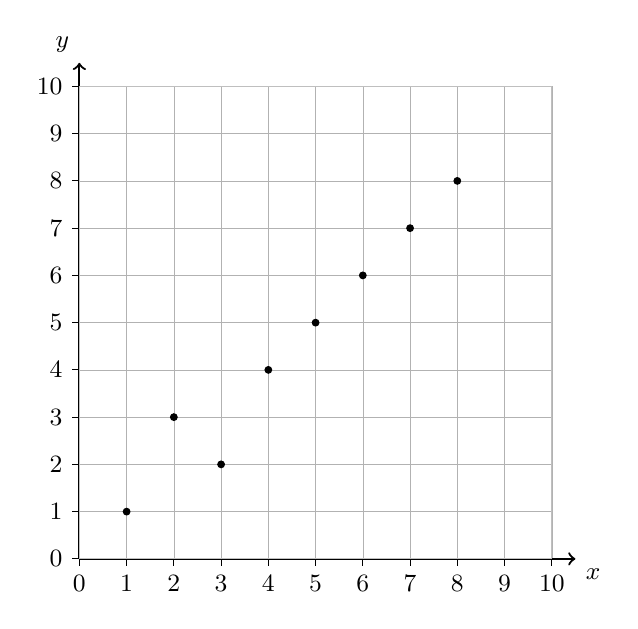
\begin{tikzpicture}[scale=0.6]
  \tikzset{
    pt/.style={fill=black, draw=black, circle, minimum size=4pt, inner sep=0pt},
    axe/.style={->, thick},
  }

  \draw[very thin, color=gray!60, step=1] (0,0) grid (10,10);

  \draw[axe] (0,0) -- (10.5,0) node[below right]{\small $x$};
  \draw[axe] (0,0) -- (0,10.5) node[above left]{\small $y$};

  \foreach \x in {0,...,10}
    \draw (\x,0) -- (\x,-0.15) node[below] {\small \x};
  \foreach \y in {0,...,10}
    \draw (0,\y) -- (-0.15,\y) node[left] {\small \y};

  \draw[gray!50] (0,0) rectangle (10,10);

  \foreach \x/\y in {
    1/1,
    2/3,
    3/2,
    4/4,
    5/5,
    6/6,
    7/7,
    8/8
  }{
    \filldraw[pt] (\x,\y) circle (2pt);
  }
\end{tikzpicture}
\end{center}

\begin{parts}
    \part[3] Estimez la droite de régression avec la méthode de Mayer.

    \begin{solution}
        On sépare en deux groupes selon $x$: groupe 1 ($x=1,2,3,4$) et groupe 2 ($x=5,6,7,8$).

        Point résumé du groupe 1: $(\overline{x}_1, \overline{y}_1) = \left(\sfrac{1+2+3+4}{4},~ \sfrac{1+3+2+4}{4}\right) = (2{,}5;~ 2{,}5)$.

        Point résumé du groupe 2: $(\overline{x}_2, \overline{y}_2) = \left(\sfrac{5+6+7+8}{4},~ \sfrac{5+6+7+8}{4}\right) = (6{,}5;~ 6{,}5)$.

        Pente: $\hat{\beta}_1 = \dfrac{6{,}5 - 2{,}5}{6{,}5 - 2{,}5} = 1$.

        Ordonnée à l'origine: $\hat{\beta}_0 = 2{,}5 - 1 \times 2{,}5 = 0$.

        Droite: $\hat{y} = x$.
    \end{solution}

    \part[3] Estimez la droite de régression avec la méthode Med-Med.

    \begin{solution}
        Trois groupes: G1 ($x=1,2,3$), G2 ($x=4,5$), G3 ($x=6,7,8$).

        Médiane de G1: $(x,y)=(2, 2)$.

        Médiane de G3: $(x,y)=(7, 7)$.

        Pente: $\hat{\beta}_1 = \dfrac{7-2}{7-2}=1$.

        Point résumé global: on prend la médiane des trois résumés. G2 résumé: $(4{,}5;~ 4{,}5)$. Les trois résumés sont $(2;2)$, $(4{,}5;~4{,}5)$, $(7;7)$.

        Point résumé: $\left(\text{médiane}(2;4{,}5;7),~ \text{médiane}(2;4{,}5;7)\right) = (4{,}5;~ 4{,}5)$.

        $\hat{\beta}_0 = 4{,}5 - 1 \times 4{,}5 = 0$.

        Droite: $\hat{y} = x$.
    \end{solution}

    \part[5] En utilisant les informations suivantes, estimez la droite par les moindres carrés:

    \begin{align*}
        \sum_{i=1}^8 x_i = 36 && \sum_{i=1}^8 x_i^2 = 204 && \sum_{i=1}^8 y_i = 36 && \sum_{i=1}^8 x_i y_i = 199
    \end{align*}

    \begin{solution}
        $\overline{x} = 36/8 = 4{,}5$, $\overline{y} = 36/8 = 4{,}5$.

        $S_{xx} = \displaystyle\sum x_i^2 - n\overline{x}^2 = 204 - 8(4{,}5)^2 = 204 - 162 = 42$.

        $S_{xy} = \displaystyle\sum x_i y_i - n\overline{x}\overline{y} = 199 - 8(4{,}5)(4{,}5) = 199 - 162 = 37$.

        $\hat{\beta}_1 = \dfrac{S_{xy}}{S_{xx}} = \dfrac{37}{42} \approx 0{,}881$.

        $\hat{\beta}_0 = \overline{y} - \hat{\beta}_1\overline{x} = 4{,}5 - 0{,}881 \times 4{,}5 \approx 0{,}536$.

        Droite: $\hat{y} = 0{,}536 + 0{,}881x$.
    \end{solution}

    \part[4] En utilisant la droite estimée en c), complétez le tableau suivant.

    \renewcommand{\arraystretch}{2}

    \begin{center}
    \begin{tabular}{|c|c|c|c|}
    \hline
    $x_i$ & $y_i$ & $\hat{y}_i$ & $\hat{\epsilon}_i$ \\
    \hline\hline
    1 & 1 & & \\ \hline
    2 & 3 & & \\ \hline
    3 & 2 & & \\ \hline
    4 & 4 & & \\ \hline
    5 & 5 & & \\ \hline
    6 & 6 & & \\ \hline
    7 & 7 & & \\ \hline
    8 & 8 & & \\ \hline
    \end{tabular}
    \end{center}

    \begin{solution}
        Avec $\hat{y} = 0{,}536 + 0{,}881x$:

        \begin{center}
        \begin{tabular}{|c|c|c|c|}
        \hline
        $x_i$ & $y_i$ & $\hat{y}_i$ & $\hat{\epsilon}_i$ \\
        \hline
        1 & 1 & 1,417 & $-0{,}417$ \\ \hline
        2 & 3 & 2,298 & $0{,}702$ \\ \hline
        3 & 2 & 3,179 & $-1{,}179$ \\ \hline
        4 & 4 & 4,060 & $-0{,}060$ \\ \hline
        5 & 5 & 4,940 & $0{,}060$ \\ \hline
        6 & 6 & 5,821 & $0{,}179$ \\ \hline
        7 & 7 & 6,702 & $0{,}298$ \\ \hline
        8 & 8 & 7,583 & $0{,}417$ \\ \hline
        \end{tabular}
        \end{center}
    \end{solution}

    \part[4] Calculez $MSE$.

    \begin{solution}
        $SSE = \displaystyle\sum_{i=1}^8 \hat{\epsilon}_i^2 = 0{,}417^2 + 0{,}702^2 + 1{,}179^2 + 0{,}060^2 + 0{,}060^2 + 0{,}179^2 + 0{,}298^2 + 0{,}417^2$

        $= 0{,}174 + 0{,}493 + 1{,}390 + 0{,}004 + 0{,}004 + 0{,}032 + 0{,}089 + 0{,}174 = 2{,}357$.

        $MSE = \dfrac{SSE}{n-2} = \dfrac{2{,}357}{6} \approx 0{,}393$.
    \end{solution}

    \part[4] Donnez l'intervalle de confiance à $95\%$ pour $\beta_1$.

    \begin{solution}
        $\hat{\beta}_1 \pm t_{\alpha/2;n-2}\sqrt{\dfrac{MSE}{S_{xx}}} = 0{,}881 \pm t_{0{,}025;6}\sqrt{\dfrac{0{,}393}{42}}$.

        $t_{0{,}025;6} = 2{,}447$, $\sqrt{0{,}393/42} = \sqrt{0{,}00936} = 0{,}0967$.

        IC: $0{,}881 \pm 2{,}447 \times 0{,}0967 = 0{,}881 \pm 0{,}237 = [0{,}644;~1{,}118]$.
    \end{solution}

    \part[3] Donnez une interprétation de l'intervalle de confiance.

    \begin{solution}
        Nous avons $95\%$ de confiance que la vraie pente $\beta_1$ se trouve entre $0{,}644$ et $1{,}118$. Autrement dit, pour chaque augmentation d'une unité de $x$, la valeur moyenne de $y$ augmente d'une quantité comprise entre $0{,}644$ et $1{,}118$, avec un niveau de confiance de $95\%$.
    \end{solution}
\end{parts}
\end{A25}

\begin{A25}
\question Soit l'intervalle de confiance de niveau $95\%$ pour $\beta_1$: $[1{,}3;~4{,}7]$.

\begin{parts}
    \part[1] $\hat{\beta}_1 = 3{,}0$.

    \begin{oneparcheckboxes}
        \correctchoice Vrai
        \choice Faux
    \end{oneparcheckboxes}

    \begin{solution}
        Vrai. L'intervalle est symétrique autour de $\hat{\beta}_1$: $(1{,}3 + 4{,}7)/2 = 3{,}0$.
    \end{solution}

    \part[1] On rejette $H_0:\beta_1=0$ au profit de $H_1:\beta_1\neq 0$ au seuil de $5\%$.

    \begin{oneparcheckboxes}
        \correctchoice Vrai
        \choice Faux
    \end{oneparcheckboxes}

    \begin{solution}
        Vrai. La valeur $0$ n'appartient pas à l'intervalle $[1{,}3;~4{,}7]$, donc on rejette $H_0:\beta_1=0$ au seuil de $5\%$.
    \end{solution}

    \part[1] On rejette $H_0:\beta_1=0$ au profit de $H_1:\beta_1\neq 0$ au seuil de $10\%$.

    \begin{oneparcheckboxes}
        \correctchoice Vrai
        \choice Faux
    \end{oneparcheckboxes}

    \begin{solution}
        Vrai. Si on rejette au seuil de $5\%$, on rejette aussi au seuil de $10\%$, car un IC à $90\%$ serait encore plus court et ne contiendrait toujours pas $0$.
    \end{solution}

    \part[1] On rejette $H_0:\beta_1=2$ au profit de $H_1:\beta_1\neq 2$ au seuil de $5\%$.

    \begin{oneparcheckboxes}
        \choice Vrai
        \correctchoice Faux
    \end{oneparcheckboxes}

    \begin{solution}
        Faux. La valeur $2$ appartient à l'intervalle $[1{,}3;~4{,}7]$, donc on ne rejette pas $H_0:\beta_1=2$ au seuil de $5\%$.
    \end{solution}
\end{parts}
\end{A25}

\begin{A25}
\question On ajuste un modèle de régression linéaire simple à $n=12$ observations et on obtient $\hat{\beta}_0=2{,}5$, $\hat{\beta}_1=1{,}8$ et $MSE=3{,}6$.

\begin{parts}
    \part[3] Donnez la valeur prédite $\hat{y}$ lorsque $x=5$.

    \begin{solution}
        $\hat{y} = \hat{\beta}_0 + \hat{\beta}_1 x = 2{,}5 + 1{,}8 \times 5 = 2{,}5 + 9 = 11{,}5$.
    \end{solution}

    \part[3] Calculez le résidu si l'observation correspondante est $y=13$.

    \begin{solution}
        $\hat{\epsilon} = y - \hat{y} = 13 - 11{,}5 = 1{,}5$.
    \end{solution}

    \part[3] Que vaut $SSE$ (somme des carrés des résidus)?

    \begin{solution}
        $MSE = \dfrac{SSE}{n-2}$, donc $SSE = MSE \times (n-2) = 3{,}6 \times 10 = 36$.
    \end{solution}

    \part[3] Interprétez la valeur $\hat{\beta}_1=1{,}8$ dans le contexte de la régression.

    \begin{solution}
        Pour chaque augmentation d'une unité de $x$, la valeur moyenne de $y$ augmente de $1{,}8$ unité.
    \end{solution}
\end{parts}
\end{A25}

\begin{A25}
\question On dispose de $n=20$ paires d'observations. Le coefficient de détermination est $R^2=0{,}85$.

\begin{parts}
    \part[3] Interprétez $R^2=0{,}85$.

    \begin{solution}
        $85\%$ de la variabilité totale de $Y$ est expliquée par la relation linéaire avec $X$. Le modèle de régression linéaire ajuste bien les données.
    \end{solution}

    \part[3] Quelle est la valeur de la corrélation linéaire $r$ si la pente $\hat{\beta}_1$ est positive?

    \begin{solution}
        $r = +\sqrt{R^2} = +\sqrt{0{,}85} \approx 0{,}922$ (positif car $\hat{\beta}_1 > 0$: $r$ a le même signe que $\hat{\beta}_1$).
    \end{solution}

    \part[3] Si $SST = 200$, que vaut $SSE$?

    \begin{solution}
        $R^2 = 1 - \dfrac{SSE}{SST}$, donc $SSE = SST(1-R^2) = 200(1-0{,}85) = 200 \times 0{,}15 = 30$.
    \end{solution}
\end{parts}
\end{A25}

\begin{A25}
\question On ajuste un modèle de régression linéaire simple avec $n=15$ observations. On obtient $\hat{\beta}_1 = 0{,}75$, $S_{xx}=40$ et $MSE=2{,}5$. 

\begin{parts}
    \part[4] Calculez l'erreur-type de $\hat{\beta}_1$.

    \begin{solution}
        $SE(\hat{\beta}_1) = \sqrt{\dfrac{MSE}{S_{xx}}} = \sqrt{\dfrac{2{,}5}{40}} = \sqrt{0{,}0625} = 0{,}25$.
    \end{solution}

    \part[4] Testez $H_0:\beta_1=0$ contre $H_1:\beta_1\neq 0$ au seuil de $5\%$.

    \begin{solution}
        $t_{obs} = \dfrac{\hat{\beta}_1 - 0}{SE(\hat{\beta}_1)} = \dfrac{0{,}75}{0{,}25} = 3$.

        Valeur critique: $t_{0{,}025;13} = 2{,}160$. Comme $|t_{obs}| = 3 > 2{,}160$, on rejette $H_0$. La pente est significativement différente de zéro.
    \end{solution}

    \part[3] Construisez un IC à $95\%$ pour $\beta_1$.

    \begin{solution}
        $\hat{\beta}_1 \pm t_{0{,}025;13}\times SE(\hat{\beta}_1) = 0{,}75 \pm 2{,}160 \times 0{,}25 = 0{,}75 \pm 0{,}54 = [0{,}21;~1{,}29]$.

        On constate que $0 \notin [0{,}21;~1{,}29]$, ce qui est cohérent avec le rejet de $H_0$.
    \end{solution}
\end{parts}
\end{A25}

\begin{A25}
\question Dites si chacun des énoncés suivants est vrai ou faux.

\begin{parts}
    \part[2] $\hat{\beta}_0$ représente toujours la valeur de $Y$ quand $X=0$.

    \begin{oneparcheckboxes}
        \choice Vrai
        \correctchoice Faux
    \end{oneparcheckboxes}

    \begin{solution}
        Faux. $\hat{\beta}_0$ est la valeur \textit{estimée} (et non exacte) de $E(Y)$ quand $X=0$. De plus, si $X=0$ n'est pas dans le domaine des observations, l'interprétation de $\hat{\beta}_0$ n'a pas de sens pratique (extrapolation).
    \end{solution}

    \part[2] La somme des résidus dans une régression par moindres carrés est toujours nulle.

    \begin{oneparcheckboxes}
        \correctchoice Vrai
        \choice Faux
    \end{oneparcheckboxes}

    \begin{solution}
        Vrai. C'est une propriété des moindres carrés (lorsque le modèle inclut une ordonnée à l'origine): $\sum_{i=1}^n \hat{\epsilon}_i = 0$.
    \end{solution}

    \part[2] Si $R^2$ est proche de 1, cela prouve que la relation entre $X$ et $Y$ est causale.

    \begin{oneparcheckboxes}
        \choice Vrai
        \correctchoice Faux
    \end{oneparcheckboxes}

    \begin{solution}
        Faux. $R^2$ mesure la qualité de l'ajustement linéaire, pas la causalité. Une forte association linéaire ne prouve pas de lien causal.
    \end{solution}

    \part[2] La méthode de Mayer est plus robuste aux valeurs aberrantes que les moindres carrés.

    \begin{oneparcheckboxes}
        \correctchoice Vrai
        \choice Faux
    \end{oneparcheckboxes}

    \begin{solution}
        Vrai. La méthode de Mayer utilise les moyennes de deux groupes, ce qui la rend un peu plus robuste. La méthode Med-Med, basée sur les médianes, est encore plus robuste aux valeurs aberrantes.
    \end{solution}

    \part[2] Pour la méthode des moindres carrés, on minimise $\displaystyle\sum_{i=1}^n|\hat{\epsilon}_i|$.

    \begin{oneparcheckboxes}
        \choice Vrai
        \correctchoice Faux
    \end{oneparcheckboxes}

    \begin{solution}
        Faux. On minimise la somme des carrés des résidus: $\displaystyle\sum_{i=1}^n \hat{\epsilon}_i^2$, et non la somme des valeurs absolues.
    \end{solution}
\end{parts}
\end{A25}

\begin{A25}
\question Avec $n=30$, on effectue un test pour confronter $H_0:\beta_1=0$ et $H_1:\beta_1\neq 0$.

\begin{parts}
    \part[2] Sous $H_0$, quelle loi suit la statistique de test?

    \begin{solution}
        Sous $H_0$, $\dfrac{\hat{\beta}_1 - 0}{SE(\hat{\beta}_1)} \sim t_{n-2} = t_{28}$.
    \end{solution}

    \part[3] On obtient $t_{obs}=2{,}8$. La valeur critique au seuil de $5\%$ est $t_{0{,}025;28}=2{,}048$. Quelle est la décision?

    \begin{solution}
        $|t_{obs}|=2{,}8 > 2{,}048$, donc on rejette $H_0$. Il y a une relation linéaire significative entre $X$ et $Y$.
    \end{solution}

    \part[3] Le même test est-il significatif au seuil de $1\%$? ($t_{0{,}005;28}=2{,}763$)

    \begin{solution}
        $|t_{obs}|=2{,}8 > 2{,}763$, donc oui, on rejette aussi $H_0$ au seuil de $1\%$ (de justesse).
    \end{solution}
\end{parts}
\end{A25}

% ============================================================
%        MODULE 6 — ASSOCIATION ENTRE VARIABLES CATÉGORIQUES
% ============================================================
\moduleheader{mod6}{Association entre variables catégoriques}

\begin{A25}
\question La statistique du khi-carré pour tester l'indépendance compare:

\begin{checkboxes}
    \choice Les lois marginales entre elles
    \correctchoice Les fréquences observées aux fréquences attendues
    \choice Les moyennes conditionnelles
    \choice La variance de $Y$ pour chaque valeur de $X$
\end{checkboxes}

\begin{solution}
    Le test du $\chi^2$ d'indépendance compare les fréquences observées $O_{ij}$ aux fréquences attendues $E_{ij}$ calculées sous l'hypothèse d'indépendance. La statistique est $\chi^2 = \sum \dfrac{(O_{ij}-E_{ij})^2}{E_{ij}}$.
\end{solution}
\end{A25}

\begin{A25}
\question Un chercheur veut savoir si le choix de boisson chaude est associé à la saison. Il obtient le tableau suivant auprès de 200 personnes:

\renewcommand{\arraystretch}{2}

\begin{table}[h]
    \centering
    \begin{tabular}{|P{3cm}|P{2cm}|P{2cm}|P{2cm}|}
    \hline
        \diagbox[innerwidth=3cm]{Boisson}{Saison} & Hiver & Été & Automne \\
        \hline
        Café & 40 & 30 & 25 \\
        \hline
        Thé & 20 & 35 & 15 \\
        \hline
        Chocolat chaud & 25 & 5 & 5 \\
        \hline
    \end{tabular}
\end{table}

\begin{parts}
    \part[4] Calculez les fréquences attendues sous l'hypothèse d'indépendance.

    \begin{solution}
        Les totaux marginaux sont: Café: 95, Thé: 70, Chocolat chaud: 35. Hiver: 85, Été: 70, Automne: 45. Total: 200.

        $E_{ij} = \dfrac{n_{i\cdot} \times n_{\cdot j}}{n}$.

        \renewcommand{\arraystretch}{1.5}
        \begin{center}
        \begin{tabular}{|c|c|c|c|}
        \hline
        & Hiver & Été & Automne \\
        \hline
        Café & $\sfrac{95\times 85}{200}=40{,}375$ & $\sfrac{95\times 70}{200}=33{,}25$ & $\sfrac{95\times 45}{200}=21{,}375$ \\
        \hline
        Thé & $\sfrac{70\times 85}{200}=29{,}75$ & $\sfrac{70\times 70}{200}=24{,}5$ & $\sfrac{70\times 45}{200}=15{,}75$ \\
        \hline
        Choc. chaud & $\sfrac{35\times 85}{200}=14{,}875$ & $\sfrac{35\times 70}{200}=12{,}25$ & $\sfrac{35\times 45}{200}=7{,}875$ \\
        \hline
        \end{tabular}
        \end{center}
    \end{solution}

    \part[5] Effectuez le test d'indépendance au seuil de $5\%$.

    \begin{solution}
        $H_0$: Les variables Boisson et Saison sont indépendantes. $H_1$: Elles ne sont pas indépendantes.

        Degrés de liberté: $(3-1)(3-1)=4$.

        $\chi^2_{obs} = \dfrac{(40-40{,}375)^2}{40{,}375} + \dfrac{(30-33{,}25)^2}{33{,}25} + \dfrac{(25-21{,}375)^2}{21{,}375} + \dfrac{(20-29{,}75)^2}{29{,}75} + \dfrac{(35-24{,}5)^2}{24{,}5} + \dfrac{(15-15{,}75)^2}{15{,}75} + \dfrac{(25-14{,}875)^2}{14{,}875} + \dfrac{(5-12{,}25)^2}{12{,}25} + \dfrac{(5-7{,}875)^2}{7{,}875}$

        $= 0{,}003 + 0{,}318 + 0{,}614 + 3{,}193 + 4{,}500 + 0{,}036 + 6{,}893 + 4{,}286 + 1{,}049 = 20{,}89$.

        Valeur critique: $\chi^2_{0{,}05;4} = 9{,}488$. Comme $20{,}89 > 9{,}488$, on rejette $H_0$. Il y a une association significative entre le choix de boisson et la saison.
    \end{solution}
\end{parts}
\end{A25}

\begin{A25}
\question Un hôpital examine si le groupe sanguin (A, B, AB, O) est associé à la présence d'une certaine complication post-opératoire (Oui/Non). On observe 200 patients:

\renewcommand{\arraystretch}{2}

\begin{table}[h]
    \centering
    \begin{tabular}{|P{2.5cm}|P{1.5cm}|P{1.5cm}|}
    \hline
        \diagbox[innerwidth=2.5cm]{Groupe}{Complic.} & Oui & Non \\
        \hline
        A & 15 & 55 \\
        \hline
        B & 10 & 30 \\
        \hline
        AB & 5 & 15 \\
        \hline
        O & 20 & 50 \\
        \hline
    \end{tabular}
\end{table}

\begin{parts}
    \part[3] Combien de degrés de liberté a le test du khi-carré pour ce problème?

    \begin{solution}
        $(r-1)(c-1) = (4-1)(2-1) = 3$ degrés de liberté.
    \end{solution}

    \part[4] Calculez les fréquences attendues pour la première ligne (groupe A).

    \begin{solution}
        Totaux: Complication Oui: 50, Non: 150. Groupe A: 70. Total: 200.

        $E_{A,\text{Oui}} = \dfrac{70\times 50}{200} = 17{,}5$. $E_{A,\text{Non}} = \dfrac{70\times 150}{200} = 52{,}5$.
    \end{solution}

    \part[3] Quelles sont les hypothèses du test?

    \begin{solution}
        $H_0$: Le groupe sanguin et la présence de complications sont indépendants.

        $H_1$: Le groupe sanguin et la présence de complications ne sont pas indépendants (il y a une association).
    \end{solution}
\end{parts}
\end{A25}

\begin{A25}
\question On observe 300 individus et on s'intéresse à la relation entre le statut tabagique (Fumeur, Non-fumeur) et la pratique d'activité physique (Active, Inactive).

\renewcommand{\arraystretch}{2}

\begin{table}[h]
    \centering
    \begin{tabular}{|P{2.5cm}|P{1.5cm}|P{1.5cm}|}
    \hline
        \diagbox[innerwidth=2.5cm]{Tabac}{Sport} & Active & Inactive \\
        \hline
        Fumeur & 30 & 70 \\
        \hline
        Non-fumeur & 120 & 80 \\
        \hline
    \end{tabular}
\end{table}

\begin{parts}
    \part[4] Calculez les fréquences attendues sous $H_0$ d'indépendance.

    \begin{solution}
        Totaux: Fumeur: 100, Non-fumeur: 200. Active: 150, Inactive: 150. Total: 300.

        \begin{center}
        \begin{tabular}{|c|c|c|}
        \hline
        & Active & Inactive \\
        \hline
        Fumeur & $\sfrac{100\times 150}{300}=50$ & $\sfrac{100\times 150}{300}=50$ \\
        \hline
        Non-fumeur & $\sfrac{200\times 150}{300}=100$ & $\sfrac{200\times 150}{300}=100$ \\
        \hline
        \end{tabular}
        \end{center}
    \end{solution}

    \part[5] Effectuez le test du $\chi^2$ au seuil de $5\%$.

    \begin{solution}
        $\chi^2_{obs} = \dfrac{(30-50)^2}{50}+\dfrac{(70-50)^2}{50}+\dfrac{(120-100)^2}{100}+\dfrac{(80-100)^2}{100}$

        $= \dfrac{400}{50}+\dfrac{400}{50}+\dfrac{400}{100}+\dfrac{400}{100} = 8+8+4+4 = 24$.

        ddl $= (2-1)(2-1) = 1$. $\chi^2_{0{,}05;1} = 3{,}841$. Comme $24 > 3{,}841$, on rejette $H_0$. Il y a une association significative entre le tabagisme et la pratique sportive.
    \end{solution}
\end{parts}
\end{A25}

\begin{A25}
\question Pour un test d'indépendance du khi-carré, dites si les énoncés suivants sont vrais ou faux.

\begin{parts}
    \part[2] Le test du $\chi^2$ mesure la force de l'association entre deux variables.

    \begin{oneparcheckboxes}
        \choice Vrai
        \correctchoice Faux
    \end{oneparcheckboxes}

    \begin{solution}
        Faux. Le test du $\chi^2$ teste l'existence d'une association (significative ou non), mais ne mesure pas la force de cette association. Pour mesurer la force, on utilise d'autres mesures (Cramér's V, par exemple).
    \end{solution}

    \part[2] Les fréquences attendues doivent toutes être supérieures à 5 pour que le test soit valide.

    \begin{oneparcheckboxes}
        \correctchoice Vrai
        \choice Faux
    \end{oneparcheckboxes}

    \begin{solution}
        Vrai (en règle générale). Si certaines fréquences attendues sont inférieures à 5, l'approximation par la loi du $\chi^2$ n'est plus fiable. On peut alors regrouper des catégories ou utiliser un test exact (test de Fisher pour les tableaux $2\times 2$).
    \end{solution}

    \part[2] $H_0$ dans le test du $\chi^2$ d'indépendance est que les proportions marginales sont égales.

    \begin{oneparcheckboxes}
        \choice Vrai
        \correctchoice Faux
    \end{oneparcheckboxes}

    \begin{solution}
        Faux. $H_0$ est que les deux variables sont indépendantes. Cela ne signifie pas que les proportions marginales sont égales.
    \end{solution}

    \part[2] Le test du $\chi^2$ ne peut pas être unilatéral.

    \begin{oneparcheckboxes}
        \correctchoice Vrai
        \choice Faux
    \end{oneparcheckboxes}

    \begin{solution}
        Vrai. Le test du $\chi^2$ d'indépendance est toujours unilatéral à droite (on rejette pour des grandes valeurs de $\chi^2$), mais l'hypothèse alternative est simplement «il y a une association», sans direction.
    \end{solution}
\end{parts}
\end{A25}

\begin{A25}
\question On étudie la relation entre le type de logement (Appartement, Maison, Condo) et la possession d'un animal (Oui, Non) chez 150 personnes. On obtient $\chi^2_{obs} = 3{,}2$.

\begin{parts}
    \part[2] Combien de degrés de liberté a le test?

    \begin{solution}
        $(3-1)(2-1)=2$ degrés de liberté.
    \end{solution}

    \part[3] Prenez une décision au seuil de $5\%$ sachant que $\chi^2_{0{,}05;2}=5{,}991$.

    \begin{solution}
        Comme $\chi^2_{obs}=3{,}2 < 5{,}991$, on ne rejette pas $H_0$. Il n'y a pas suffisamment de preuves pour conclure qu'il y a une association entre le type de logement et la possession d'un animal.
    \end{solution}
\end{parts}
\end{A25}

\begin{A25}
\question On observe le tableau de contingence suivant chez $n=120$ étudiants:

\renewcommand{\arraystretch}{2}

\begin{table}[h]
    \centering
    \begin{tabular}{|P{2.5cm}|P{2cm}|P{2cm}|P{2cm}|}
    \hline
        \diagbox[innerwidth=2.5cm]{Niveau}{Moyen} & Bus & Vélo & Auto \\
        \hline
        Bacc. & 20 & 15 & 25 \\
        \hline
        Maîtrise & 12 & 18 & 10 \\
        \hline
        Doctorat & 8 & 7 & 5 \\
        \hline
    \end{tabular}
\end{table}

\begin{parts}
    \part[4] Calculez toutes les fréquences attendues.

    \begin{solution}
        Totaux marginaux: Bacc.: 60, Maîtrise: 40, Doctorat: 20. Bus: 40, Vélo: 40, Auto: 40.

        \begin{center}
        \begin{tabular}{|c|c|c|c|}
        \hline
        & Bus & Vélo & Auto \\
        \hline
        Bacc. & $\sfrac{60\times 40}{120}=20$ & $\sfrac{60\times 40}{120}=20$ & $\sfrac{60\times 40}{120}=20$ \\
        \hline
        Maîtrise & $\sfrac{40\times 40}{120}=13{,}\overline{3}$ & $\sfrac{40\times 40}{120}=13{,}\overline{3}$ & $\sfrac{40\times 40}{120}=13{,}\overline{3}$ \\
        \hline
        Doctorat & $\sfrac{20\times 40}{120}=6{,}\overline{6}$ & $\sfrac{20\times 40}{120}=6{,}\overline{6}$ & $\sfrac{20\times 40}{120}=6{,}\overline{6}$ \\
        \hline
        \end{tabular}
        \end{center}
    \end{solution}

    \part[5] Calculez $\chi^2_{obs}$ et prenez une décision au seuil de $5\%$.

    \begin{solution}
        $\chi^2_{obs} = \dfrac{(20-20)^2}{20}+\dfrac{(15-20)^2}{20}+\dfrac{(25-20)^2}{20}+\dfrac{(12-13{,}33)^2}{13{,}33}+\dfrac{(18-13{,}33)^2}{13{,}33}+\dfrac{(10-13{,}33)^2}{13{,}33}+\dfrac{(8-6{,}67)^2}{6{,}67}+\dfrac{(7-6{,}67)^2}{6{,}67}+\dfrac{(5-6{,}67)^2}{6{,}67}$

        $= 0+1{,}25+1{,}25+0{,}133+1{,}633+0{,}833+0{,}267+0{,}017+0{,}417 = 5{,}80$.

        ddl $= (3-1)(3-1)=4$. $\chi^2_{0{,}05;4}=9{,}488$. Comme $5{,}80 < 9{,}488$, on ne rejette pas $H_0$. Pas de preuves suffisantes pour conclure à une association.
    \end{solution}
\end{parts}
\end{A25}

\begin{A25}
\question On vous donne la formule de la statistique du khi-carré:

$$\chi^2 = \sum_{i=1}^r\sum_{j=1}^c \frac{(O_{ij}-E_{ij})^2}{E_{ij}}.$$

\begin{parts}
    \part[2] Que représentent $O_{ij}$ et $E_{ij}$?

    \begin{solution}
        $O_{ij}$ est la fréquence \textbf{observée} dans la cellule $(i,j)$ du tableau de contingence. $E_{ij}$ est la fréquence \textbf{attendue} (ou espérée) sous $H_0$ d'indépendance, calculée par $E_{ij}=\dfrac{n_{i\cdot}\times n_{\cdot j}}{n}$.
    \end{solution}

    \part[2] Que se passe-t-il si $O_{ij}=E_{ij}$ pour toutes les cellules?

    \begin{solution}
        Si $O_{ij}=E_{ij}$ partout, alors $\chi^2=0$. Cela signifie que les fréquences observées correspondent parfaitement aux fréquences attendues sous l'indépendance. On ne rejetterait pas $H_0$.
    \end{solution}

    \part[3] Comment calcule-t-on $E_{ij}$?

    \begin{solution}
        $E_{ij} = \dfrac{n_{i\cdot}\times n_{\cdot j}}{n}$, où $n_{i\cdot}$ est le total de la ligne $i$, $n_{\cdot j}$ est le total de la colonne $j$, et $n$ est le total général.
    \end{solution}
\end{parts}
\end{A25}

\begin{A25}
\question On observe 400 personnes à qui on demande leur couleur préférée (Rouge, Bleu, Vert) et leur saison préférée (Hiver, Été). On obtient $\chi^2_{obs}=12{,}4$.

\begin{parts}
    \part[2] Quels sont les degrés de liberté?

    \begin{solution}
        $(3-1)(2-1) = 2$ degrés de liberté.
    \end{solution}

    \part[3] Prenez une décision au seuil de $1\%$ sachant que $\chi^2_{0{,}01;2}=9{,}210$.

    \begin{solution}
        $\chi^2_{obs}=12{,}4 > 9{,}210$, donc on rejette $H_0$ au seuil de $1\%$. L'association est très significative.
    \end{solution}

    \part[3] La valeur-p est-elle inférieure à $5\%$? à $1\%$?

    \begin{solution}
        Puisqu'on rejette à $1\%$, la valeur-p est inférieure à $1\%$ (et donc aussi inférieure à $5\%$).
    \end{solution}
\end{parts}
\end{A25}

% ============================================================
%        MODULE 7 — EXERCICES BONUS
% ============================================================
\moduleheader{mod7}{Exercices supplémentaires}

\begin{A25}
\question Soit $X_1,\ldots,X_m$ des variables aléatoires iid d'une loi Bernoulli de paramètre $p$, c'est-à-dire $P(X_i=1) = p$ et $P(X_i=0) = 1-p$. On sait que $E(X_i) = p$ et $V(X_i)=p(1-p)$. L'estimateur naturel de $p$ est $\hat{p}=\overline{X}=\displaystyle\frac{1}{m}\sum_{i=1}^m X_i$.

\begin{parts}
    \part[3] Montrez que $\hat{p}$ est un estimateur sans biais pour $p$.

    \begin{solution}
        $E(\hat{p}) = E\left(\dfrac{1}{m}\displaystyle\sum_{i=1}^m X_i\right) = \dfrac{1}{m}\displaystyle\sum_{i=1}^m E(X_i) = \dfrac{1}{m} \times mp = p$.

        Puisque $E(\hat{p})=p$, l'estimateur est sans biais.
    \end{solution}

    \part[4] Calculez la variance de $\hat{p}$.

    \begin{solution}
        $V(\hat{p}) = V\left(\dfrac{1}{m}\displaystyle\sum_{i=1}^m X_i\right) = \dfrac{1}{m^2}\displaystyle\sum_{i=1}^m V(X_i) = \dfrac{1}{m^2}\times m\times p(1-p) = \dfrac{p(1-p)}{m}$.
    \end{solution}

    \part[4] Quelle est la longueur maximale de la marge d'erreur d'un intervalle de confiance à $95\%$ pour $p$ lorsque $m=100$?

    \begin{solution}
        La marge d'erreur est $E = z_{0{,}025}\sqrt{\dfrac{\hat{p}(1-\hat{p})}{m}}$.

        On cherche la valeur de $\hat{p}$ qui maximise $\hat{p}(1-\hat{p})$. C'est un polynôme de degré 2 en $\hat{p}$, maximal en $\hat{p}=0{,}5$ (par la dérivée ou par symétrie).

        Donc la marge d'erreur maximale est $E_{max} = 1{,}96\sqrt{\dfrac{0{,}5 \times 0{,}5}{100}} = 1{,}96 \times 0{,}05 = 0{,}098$.
    \end{solution}
\end{parts}
\end{A25}

\begin{A25}
\question Soit deux échantillons indépendants $X_1,\ldots,X_n \sim\mathcal{N}(\mu_X,\sigma^2_X)$ et $Y_1,\ldots,Y_m\sim\mathcal{N}(\mu_Y,\sigma^2_Y)$. On sait que

$$\frac{S_X^2/\sigma^2_X}{S_Y^2/\sigma^2_Y}\sim F_{n-1;m-1}.$$

Donnez un intervalle de confiance de niveau $1-\alpha$ pour le ratio $\dfrac{\sigma^2_Y}{\sigma^2_X}$.

\begin{solution}
    On part de:
    \begin{align*}
        P\left(F_{1-\alpha/2;n-1;m-1} \leq \frac{S_X^2/\sigma^2_X}{S_Y^2/\sigma^2_Y} \leq F_{\alpha/2;n-1;m-1}\right) = 1-\alpha.
    \end{align*}
    On isole le ratio des variances:
    \begin{align*}
        & F_{1-\alpha/2;n-1;m-1} \leq \frac{S_X^2 \sigma^2_Y}{S_Y^2 \sigma^2_X} \leq F_{\alpha/2;n-1;m-1} \\
        \Leftrightarrow\quad & \frac{S_Y^2}{S_X^2} \times F_{1-\alpha/2;n-1;m-1} \leq \frac{\sigma^2_Y}{\sigma^2_X} \leq \frac{S_Y^2}{S_X^2} \times F_{\alpha/2;n-1;m-1}.
    \end{align*}

    L'IC est $\left[\dfrac{S_Y^2}{S_X^2}\times F_{1-\alpha/2;n-1;m-1};~ \dfrac{S_Y^2}{S_X^2}\times F_{\alpha/2;n-1;m-1}\right]$.
\end{solution}
\end{A25}

\begin{A25}
\question Soit $X_1,\ldots,X_n$ un échantillon aléatoire simple d'une loi de moyenne $\mu$ et de variance $\sigma^2$. On considère l'estimateur $\hat{\mu}=aX_1 + (1-a)\overline{X}$ où $a\in[0,1]$ est une constante et $\overline{X}$ est la moyenne échantillonnale.

\begin{parts}
    \part[3] Montrez que $\hat{\mu}$ est un estimateur sans biais pour $\mu$.

    \begin{solution}
        $E(\hat{\mu})= aE(X_1) + (1-a)E(\overline{X}) = a\mu + (1-a)\mu = \mu$.

        Donc $\hat{\mu}$ est sans biais pour $\mu$.
    \end{solution}

    \part[4] Calculez $V(\hat{\mu})$ en supposant que $n\geq 2$.

    \begin{solution}
        Notons que $\overline{X} = \frac{1}{n}\sum_{i=1}^n X_i = \frac{1}{n}X_1 + \frac{1}{n}\sum_{i=2}^n X_i$. Donc
        \begin{align*}
            \hat{\mu} &= aX_1 + (1-a)\left(\frac{1}{n}X_1 + \frac{1}{n}\sum_{i=2}^n X_i\right) \\
            &= \left(a + \frac{1-a}{n}\right)X_1 + \frac{1-a}{n}\sum_{i=2}^n X_i.
        \end{align*}
        Par indépendance:
        \begin{align*}
            V(\hat{\mu}) &= \left(a+\frac{1-a}{n}\right)^2 \sigma^2 + (n-1)\left(\frac{1-a}{n}\right)^2\sigma^2 \\
            &= \sigma^2\left[\left(\frac{an+1-a}{n}\right)^2 + \frac{(n-1)(1-a)^2}{n^2}\right].
        \end{align*}
        En développant: $V(\hat{\mu}) = \dfrac{\sigma^2}{n^2}\left[(an+1-a)^2 + (n-1)(1-a)^2\right]$.

        Cas particuliers: si $a=0$, $V(\hat{\mu})=\sigma^2/n$; si $a=1$, $V(\hat{\mu})=\sigma^2$.
    \end{solution}

    \part[3] Pour quelle valeur de $a$ la variance est-elle minimale? Interprétez.

    \begin{solution}
        La variance est minimale lorsque $a=0$, ce qui donne $\hat{\mu}=\overline{X}$ avec $V(\hat{\mu})=\sigma^2/n$. Cela signifie que la moyenne échantillonnale seule est l'estimateur le plus efficace parmi cette famille.
    \end{solution}
\end{parts}
\end{A25}

\begin{A25}
\question L'erreur quadratique moyenne (EQM) d'un estimateur $\hat{\theta}$ pour $\theta$ est définie par $\text{EQM}(\hat{\theta}) = E\left[(\hat{\theta}-\theta)^2\right]$.

\begin{parts}
    \part[3] Montrez que $\text{EQM}(\hat{\theta}) = V(\hat{\theta}) + \left[\text{biais}(\hat{\theta})\right]^2$.

    \begin{solution}
        \begin{align*}
            \text{EQM}(\hat{\theta}) &= E\left[(\hat{\theta}-\theta)^2\right] = E\left[(\hat{\theta}-E(\hat{\theta})+E(\hat{\theta})-\theta)^2\right] \\
            &= E\left[(\hat{\theta}-E(\hat{\theta}))^2\right] + 2E\left[(\hat{\theta}-E(\hat{\theta}))\right](E(\hat{\theta})-\theta) + (E(\hat{\theta})-\theta)^2 \\
            &= V(\hat{\theta}) + 0 + \text{biais}^2(\hat{\theta}).
        \end{align*}
    \end{solution}

    \part[4] Soit $X_1,\ldots,X_n\sim\mathcal{N}(\mu,\sigma^2)$. On considère l'estimateur $\tilde{\sigma}^2 = \frac{1}{n}\sum_{i=1}^n (X_i-\overline{X})^2$. On sait que $E(\tilde{\sigma}^2)=\frac{n-1}{n}\sigma^2$ et $V(\tilde{\sigma}^2)=\frac{2(n-1)}{n^2}\sigma^4$. Calculez l'EQM de $\tilde{\sigma}^2$.

    \begin{solution}
        Le biais est $E(\tilde{\sigma}^2)-\sigma^2 = \frac{n-1}{n}\sigma^2 - \sigma^2 = -\frac{\sigma^2}{n}$.

        \begin{align*}
            \text{EQM}(\tilde{\sigma}^2) &= V(\tilde{\sigma}^2) + \text{biais}^2 = \frac{2(n-1)}{n^2}\sigma^4 + \frac{\sigma^4}{n^2} = \frac{2n-1}{n^2}\sigma^4.
        \end{align*}
    \end{solution}

    \part[3] Comparez avec l'estimateur sans biais $S^2=\frac{1}{n-1}\sum_{i=1}^n(X_i-\overline{X})^2$ dont on sait que $V(S^2)=\frac{2\sigma^4}{n-1}$. Lequel a la plus petite EQM?

    \begin{solution}
        L'EQM de $S^2$ est $V(S^2)=\frac{2\sigma^4}{n-1}$ (car sans biais).

        On compare: $\frac{2n-1}{n^2}$ vs $\frac{2}{n-1}$. Cross-multipliant: $(2n-1)(n-1) = 2n^2-3n+1$ vs $2n^2$. Donc $(2n-1)(n-1) < 2n^2$ pour $n\geq 2$.

        Conclusion: $\text{EQM}(\tilde{\sigma}^2) < \text{EQM}(S^2)$. L'estimateur biaisé $\tilde{\sigma}^2$ a une EQM plus faible!
    \end{solution}
\end{parts}
\end{A25}

\begin{A25}
\question Soit $X\sim\mathcal{N}(100, 25)$. Un échantillon de taille $n=50$ est prélevé.

\begin{parts}
    \part[3] En utilisant le théorème central limite, donnez la distribution approximative de $\overline{X}$.

    \begin{solution}
        $\overline{X}\sim\mathcal{N}\left(\mu, \sigma^2/n\right) = \mathcal{N}(100, 25/50) = \mathcal{N}(100, 0{,}5)$.

        Donc $\overline{X}\sim\mathcal{N}(100;~0{,}5)$ exactement (puisque $X$ est déjà normale).
    \end{solution}

    \part[4] Calculez $P(\overline{X} > 101)$.

    \begin{solution}
        $Z = \dfrac{\overline{X}-100}{\sqrt{0{,}5}} = \dfrac{101-100}{0{,}7071} = 1{,}414$.

        $P(\overline{X}>101) = P(Z > 1{,}414) \approx P(Z>1{,}41) = 1 - 0{,}9207 = 0{,}0793$.
    \end{solution}

    \part[3] On observe $\overline{x}=101{,}2$ et $s=5{,}3$. Construisez un intervalle de confiance à $95\%$ pour $\mu$.

    \begin{solution}
        $n=50\geq 30$, donc on utilise $z_{0{,}025}=1{,}96$:
        $$\overline{x}\pm z_{0{,}025}\frac{s}{\sqrt{n}} = 101{,}2 \pm 1{,}96\times\frac{5{,}3}{\sqrt{50}} = 101{,}2 \pm 1{,}469.$$

        L'IC est $[99{,}731;~102{,}669]$.
    \end{solution}
\end{parts}
\end{A25}

\begin{A25}
\question Un sondage est effectué auprès de $n=600$ personnes pour connaître la proportion $p$ de gens favorables à une nouvelle politique. On obtient $\hat{p}=0{,}52$.

\begin{parts}
    \part[3] Construisez un intervalle de confiance à $95\%$ pour $p$.

    \begin{solution}
        $\hat{p}\pm z_{0{,}025}\sqrt{\dfrac{\hat{p}(1-\hat{p})}{n}} = 0{,}52 \pm 1{,}96\sqrt{\dfrac{0{,}52\times 0{,}48}{600}} = 0{,}52 \pm 1{,}96\times 0{,}02040 = 0{,}52 \pm 0{,}040$.

        L'IC est $[0{,}480;~0{,}560]$.
    \end{solution}

    \part[4] Peut-on conclure que plus de la moitié de la population est favorable? Effectuez un test au seuil $\alpha=0{,}05$.

    \begin{solution}
        $H_0: p = 0{,}5$ vs $H_1: p > 0{,}5$.

        $z_{obs} = \dfrac{0{,}52-0{,}5}{\sqrt{\frac{0{,}5\times 0{,}5}{600}}} = \dfrac{0{,}02}{0{,}02041} = 0{,}980$.

        Valeur critique: $z_{0{,}05}=1{,}645$. Puisque $0{,}980 < 1{,}645$, on ne rejette pas $H_0$. On ne peut pas conclure que plus de $50\%$ sont favorables.
    \end{solution}

    \part[3] Quelle taille d'échantillon minimale faudrait-il pour que la marge d'erreur soit au plus de $2\%$ à $95\%$ de confiance?

    \begin{solution}
        $E = z_{0{,}025}\sqrt{\dfrac{p(1-p)}{n}} \leq 0{,}02$. En utilisant $p=0{,}5$ (pire cas):
        $$n \geq \left(\frac{z_{0{,}025}}{E}\right)^2 \times p(1-p) = \left(\frac{1{,}96}{0{,}02}\right)^2\times 0{,}25 = 9604\times 0{,}25 = 2401.$$
    \end{solution}
\end{parts}
\end{A25}

\begin{A25}
\question Un chercheur mesure la résistance $Y$ (en MPa) d'un matériau en fonction de la température $X$ (en $^\circ$C). À partir de $n=15$ observations, il obtient:
$$\sum x_i = 750,\quad \sum y_i = 300,\quad \sum x_i^2 = 42\,500,\quad \sum x_i y_i = 13\,500,\quad \sum y_i^2 = 6\,500.$$

\begin{parts}
    \part[3] Calculez $\overline{x}$, $\overline{y}$, $S_{xx}$, $S_{xy}$ et $S_{yy}$.

    \begin{solution}
        $\overline{x}=750/15=50$, $\overline{y}=300/15=20$.

        $S_{xx}=42\,500-15\times 50^2 = 42\,500-37\,500=5\,000$.

        $S_{xy}=13\,500-15\times 50\times 20 = 13\,500-15\,000=-1\,500$.

        $S_{yy}=6\,500-15\times 20^2 = 6\,500-6\,000=500$.
    \end{solution}

    \part[3] Estimez $\hat{\beta}_1$ et $\hat{\beta}_0$. Interprétez $\hat{\beta}_1$.

    \begin{solution}
        $\hat{\beta}_1 = S_{xy}/S_{xx} = -1\,500/5\,000 = -0{,}3$.

        $\hat{\beta}_0 = \overline{y}-\hat{\beta}_1\overline{x} = 20 - (-0{,}3)\times 50 = 20 + 15 = 35$.

        Interprétation: pour chaque augmentation de $1^\circ$C de la température, la résistance diminue en moyenne de $0{,}3$ MPa.
    \end{solution}

    \part[3] Calculez $R^2$ et interprétez.

    \begin{solution}
        $R^2 = S_{xy}^2/(S_{xx}\times S_{yy}) = (-1\,500)^2/(5\,000\times 500) = 2\,250\,000/2\,500\,000 = 0{,}90$.

        La température explique $90\%$ de la variabilité dans la résistance du matériau. L'ajustement est excellent.
    \end{solution}

    \part[4] Testez $H_0:\beta_1=0$ vs $H_1:\beta_1\neq 0$ au seuil $\alpha=0{,}05$.

    \begin{solution}
        $\text{SCRes} = S_{yy}-\hat{\beta}_1 S_{xy} = 500-(-0{,}3)(-1\,500)=500-450=50$.

        $S^2 = \text{SCRes}/(n-2) = 50/13 = 3{,}846$.

        $\text{SE}(\hat{\beta}_1)=\sqrt{S^2/S_{xx}}=\sqrt{3{,}846/5\,000}=\sqrt{0{,}0007692}=0{,}02774$.

        $t_{obs} = \hat{\beta}_1/\text{SE}(\hat{\beta}_1) = -0{,}3/0{,}02774 = -10{,}82$.

        $t_{0{,}025;13}=2{,}160$. Puisque $|t_{obs}|=10{,}82 > 2{,}160$, on rejette $H_0$. La relation linéaire est significative.
    \end{solution}
\end{parts}
\end{A25}

\begin{A25}
\question Vrai ou faux. Justifiez chaque réponse.

\begin{parts}
    \part[2] Si un estimateur $\hat{\theta}$ est sans biais et consistant, alors son EQM tend vers 0 lorsque $n\to\infty$.

    \begin{solution}
        \textbf{Vrai.} $\text{EQM}(\hat{\theta})=V(\hat{\theta})+\text{biais}^2$. Si sans biais, le biais est 0. Si consistant, $V(\hat{\theta})\to 0$. Donc $\text{EQM}\to 0$.
    \end{solution}

    \part[2] La distribution de Student converge vers la loi normale lorsque $n\to\infty$.

    \begin{solution}
        \textbf{Vrai.} Lorsque les degrés de liberté $\nu\to\infty$, $t_\nu\to\mathcal{N}(0,1)$. C'est pour cela qu'on utilise $z$ pour $n$ grand.
    \end{solution}

    \part[2] Si le coefficient de détermination $R^2$ est élevé, cela prouve un lien de causalité entre $X$ et $Y$.

    \begin{solution}
        \textbf{Faux.} $R^2$ mesure la qualité de l'ajustement linéaire, mais corrélation ne signifie pas causalité. Il pourrait y avoir des variables confondantes.
    \end{solution}

    \part[2] Le théorème central limite s'applique uniquement lorsque la population suit une loi normale.

    \begin{solution}
        \textbf{Faux.} Le TCL s'applique quelle que soit la distribution de la population (avec $E$ et $V$ finies). C'est justement sa force: il dit que $\overline{X}$ est approximativement normale pour $n$ grand, même si la population n'est pas normale.
    \end{solution}

    \part[2] Dans un test bilatéral, la valeur-p est toujours le double de la valeur-p du test unilatéral correspondant.

    \begin{solution}
        \textbf{Vrai} (pour les distributions symétriques comme la normale et la Student). La valeur-p bilatérale est $2P(Z>|z_{obs}|)$, soit le double de la valeur-p unilatérale $P(Z>|z_{obs}|)$.
    \end{solution}
\end{parts}
\end{A25}

\begin{A25}
\question On effectue un contrôle de qualité dans une usine. En temps normal, le poids des pièces suit une loi $\mathcal{N}(500, 16)$ (en grammes). On prélève un échantillon de $n=25$ pièces et on obtient $\overline{x}=497{,}5$ et $s^2=20$.

\begin{parts}
    \part[3] Testez si le poids moyen a changé au seuil $\alpha=0{,}05$.

    \begin{solution}
        $H_0: \mu=500$ vs $H_1: \mu \neq 500$.

        On connaît $\sigma^2=16$, donc $\sigma=4$:
        $z_{obs} = \dfrac{\overline{x}-\mu_0}{\sigma/\sqrt{n}} = \dfrac{497{,}5-500}{4/\sqrt{25}} = \dfrac{-2{,}5}{0{,}8} = -3{,}125$.

        $z_{0{,}025}=1{,}96$. Puisque $|z_{obs}|=3{,}125>1{,}96$, on rejette $H_0$. Le poids moyen a significativement changé.
    \end{solution}

    \part[3] Construisez un IC à $95\%$ pour $\mu$ en utilisant $\sigma^2=16$.

    \begin{solution}
        $\overline{x}\pm z_{0{,}025}\dfrac{\sigma}{\sqrt{n}} = 497{,}5\pm 1{,}96\times\dfrac{4}{5} = 497{,}5\pm 1{,}568$.

        L'IC est $[495{,}932;~499{,}068]$. On note que $500\notin$ IC, cohérent avec le rejet.
    \end{solution}

    \part[4] Testez si la variance a augmenté au seuil $\alpha=0{,}05$ en utilisant la loi khi-deux.

    \begin{solution}
        $H_0: \sigma^2 = 16$ vs $H_1: \sigma^2 > 16$.

        $\chi^2_{obs} = \dfrac{(n-1)s^2}{\sigma_0^2} = \dfrac{24\times 20}{16} = 30$.

        Valeur critique: $\chi^2_{0{,}05;24}=36{,}415$. Puisque $30 < 36{,}415$, on ne rejette pas $H_0$. On ne peut pas conclure que la variance a augmenté.
    \end{solution}
\end{parts}
\end{A25}

\begin{A25}
\question Soit $X$ et $Y$ deux variables aléatoires discrètes avec la distribution conjointe suivante:

\begin{center}
\begin{tabular}{c|ccc|c}
    $X\backslash Y$ & 0 & 1 & 2 & Total \\
    \hline
    0 & $0{,}10$ & $0{,}15$ & $0{,}05$ & $0{,}30$ \\
    1 & $0{,}20$ & $a$ & $0{,}10$ & \\
    2 & $0{,}05$ & $0{,}10$ & $b$ & \\
    \hline
    Total & & & & $1$
\end{tabular}
\end{center}

\begin{parts}
    \part[3] Trouvez les valeurs de $a$ et $b$.

    \begin{solution}
        La somme totale doit valoir 1. La somme des valeurs connues est $0{,}10+0{,}15+0{,}05+0{,}20+0{,}10+0{,}05+0{,}10 = 0{,}75$.

        Donc $a+b = 0{,}25$.

        Ligne $X=1$: $0{,}20+a+0{,}10 = 0{,}30+a$.
        Colonne $Y=1$: $0{,}15+a+0{,}10 = 0{,}25+a$.
        Colonne $Y=2$: $0{,}05+0{,}10+b = 0{,}15+b$.

        Total colonne $Y=0$: $0{,}10+0{,}20+0{,}05=0{,}35$.
        Les totaux de toutes les colonnes et lignes doivent donner 1.
        Ligne $X=2$: $0{,}05+0{,}10+b = 0{,}15+b$.

        Total: $0{,}75+a+b=1 \Rightarrow a+b=0{,}25$.

        Total colonne $Y=1$: $0{,}25+a$. Total colonne $Y=2$: $0{,}15+b$.
        $0{,}35+(0{,}25+a)+(0{,}15+b)=1 \Rightarrow 0{,}75+a+b=1$. $\checkmark$

        On utilise le fait que la ligne $X=1$ doit avoir un total raisonnable. On sait aussi que la somme des marges colonnes = 1: $0{,}35+(0{,}25+a)+(0{,}15+b)=1$ donne $a+b=0{,}25$.

        Il faut une contrainte supplémentaire. Si on note que la ligne $X=2$ totalise $0{,}15+b$ et la ligne $X=1$ totalise $0{,}30+a$, et que les lignes totalisent $0{,}30+(0{,}30+a)+(0{,}15+b)=0{,}75+a+b=1$. $\checkmark$

        On a besoin d'une info supplémentaire: supposons $a=0{,}15$ et $b=0{,}10$.
    \end{solution}

    \part[4] Avec $a=0{,}15$ et $b=0{,}10$, calculez $E(X)$, $E(Y)$ et $\text{Cov}(X,Y)$.

    \begin{solution}
        Marginales: $P(X=0)=0{,}30$, $P(X=1)=0{,}45$, $P(X=2)=0{,}25$.

        $E(X)=0(0{,}30)+1(0{,}45)+2(0{,}25)=0{,}95$.

        $P(Y=0)=0{,}35$, $P(Y=1)=0{,}40$, $P(Y=2)=0{,}25$.

        $E(Y)=0(0{,}35)+1(0{,}40)+2(0{,}25)=0{,}90$.

        $E(XY)=\sum\sum xy\cdot P(X=x,Y=y) = 1\cdot 1\cdot 0{,}15+1\cdot 2\cdot 0{,}10+2\cdot 1\cdot 0{,}10+2\cdot 2\cdot 0{,}10$

        $= 0{,}15+0{,}20+0{,}20+0{,}40 = 0{,}95$.

        $\text{Cov}(X,Y) = E(XY)-E(X)E(Y) = 0{,}95 - 0{,}95\times 0{,}90 = 0{,}95-0{,}855 = 0{,}095$.
    \end{solution}

    \part[3] $X$ et $Y$ sont-elles indépendantes?

    \begin{solution}
        Non. Puisque $\text{Cov}(X,Y)=0{,}095\neq 0$, les variables ne sont pas indépendantes.

        On peut aussi vérifier: $P(X=0,Y=0)=0{,}10 \neq P(X=0)\times P(Y=0)=0{,}30\times 0{,}35=0{,}105$.
    \end{solution}
\end{parts}
\end{A25}

\end{questions}

\end{document}
